\documentclass[twoside]{supsistudent} 
\usepackage{url}
\usepackage{pdfpages} 
%\usepackage{mermaid}

\setlength{\parindent}{0pt}


\newcommand{\problemchapter}[1]{%
  \chapter*{#1}%
  \addcontentsline{toc}{chapter}{#1}%
\markboth{#1}{#1}
}

% Numerazione delle appendici secondo norma
\addto\appendix{
\renewcommand{\thesection}{\Alph{chapter}.\arabic{section}}
\renewcommand{\thesubsection}{\thesection.\arabic{subsection}}}

\setcounter{secnumdepth}{5} 	%per avere più livelli nei titoli
\setcounter{tocdepth}{5}		%per avere più livelli nell'indice


\titolo{Sviluppo applicazione cloud-native a scopo didattico}
\studente{Nicola Romano}
\relatore{Massimo Coluzzi}
\correlatore{Roberto Guidi}
\committente{SUPSI}
\corso{Ingegneria informatica}
\modulo{Progetto di diploma}
\anno{2026}



\begin{document}

\pagenumbering{alph}
\maketitle
\onehalfspacing
\frontmatter

\cleardoublepage
\vspace*{0.2\textheight}
\begin{flushright}
\textit{A mio nonno Franco}
\end{flushright}
\vfill
\cleardoublepage

\chapter{Abstract}
\section{English}
This thesis presents a practical case study for DevOps education at SUPSI, demonstrating the progressive evolution of a Spring Boot monolith into a distributed, cloud-native microservices platform. Across six milestones, the compute-intensive AI and image processing application integrates Docker containerization, Kubernetes orchestration, Kafka-mediated asynchronous scaling, Keycloak identity management, and CI/CD automation. The result validates modern architectural orchestration principles.  
\section{Italiano}
Questa tesi presenta un caso di studio pratico per la formazione in ambito DevOps nel contesto della SUPSI, dimostrando la progressiva evoluzione di un monolite SpringBoot in una piattaforma distribuita, cloud-native e basata su microservizi. Attraverso sei milestone ,l'applicazione di IA e elaborazione immagini integra containerizzazione Docker, orchestrazione Kubernetes, scaling asincrono tramite Kafka, gestione identità con Keycloak e automazione CI/CD. Il risultato convalida i moderni principi di orchestrazione architetturale.

\section{Use of AI}
Generative AI tools (primarily Claude, used through a persistent project workspace rather than disposable chat sessions) were used throughout this thesis, under a deliberate human-in-the-loop approach whose guiding principle was preserving ownership and understanding of the resulting system, rather than delegating its production. No autonomous coding agent was used at any point: AI-authored code was never applied directly to the repository. Every suggestion was read, understood, adapted where necessary, and committed by hand, so that all the code remained under the author ownership and every design decision could be explained and justified if required. Auxiliary, narrower-scope cloud AI services were occasionally used outside this main workspace for isolated debugging questions or one-off syntax lookups, where no architectural context needed to be carried over between turns.

In coding and architectural decision-making, AI was used as a discussion partner rather than a source of ready-made answers: proposing implementation options, surfacing trade-offs between them (for instance, the Alpine-versus-Debian-slim base image decision in Chapter \emph{Results}, Section \emph{Containerization}, or the storage-key-ownership question revisited during the Kafka integration), and reviewing already written code  for bugs or omissions. The iterative, milestone-by-milestone structure of the project described in Chapter \emph{Approach} was itself well suited to this mode of use: each milestone's scope was narrow enough that AI-assisted exploration of a design space could be followed immediately by manual implementation and validation, rather than accumulating unreviewed, AI-generated surface area across an entire milestone at once.

For research, AI (primarily Claude and Anara) was used to gain insights quickly within an unfamiliar topic, for example, summarizing the trade-offs between Kafka and RabbitMQ, or the practical differences between Istio and Linkerd, before deeper reading. It was not treated as a primary source in its own right: claims relevant to the State of the Art chapter were checked against official documentation, vendor sources, or the peer-reviewed literature cited there, rather than taken on the AI's word alone. This same tool was also used to locate and shortlist candidate academic references on request, but still requiring verification of each source's actual content and relevance before citing it.

For documentation, AI assisted in producing the markdown sprint recaps that accompany each milestone and in drafting and editing sections of this LaTeX report, restructuring prose, tightening explanations, and helping translate the sprint recaps' implementation-level detail into the report's narrative structure. As with the code, every generated passage was reviewed against what was actually built (the manifests, the source code, the validation scripts) before being retained, so that the report's technical claims trace back to the implementation itself rather than to an AI-generated approximation of it.

\problemchapter{Ringraziamenti}
Desidero cogliere questa occasione per ringraziare tutti coloro che mi hanno supportato e motivato durante il mio percorso universitario e, in particolare, durante la stesura di questa tesi.
Un ringraziamento speciale va al mio relatore Massimo Coluzzi, e al mio corelatore, Roberto Guidi, che, per la loro costante disponibilità e il prezioso supporto tecnico, sono stati fondamentali. Li ringrazio inoltre per aver incoraggiato e accolto le mie idee, rendendole attuabili all'interno di questo progetto di diploma.
Vorrei esprimere la mia più profonda gratitudine alla mia famiglia: a mia madre Jacqueline, mio padre Giulio e a mia sorella Carola. Grazie per avermi sempre auitato e sostenuto durante questi anni di studio.
Infine, un ringraziamento di cuore va a tutti gli amici che mi sono stati vicini lungo questo cammino e durante il periodo di lavoro dedicato alla tesi: Alessio, Andrea, Antonio, Diego, Giorgio, Guymarie, Lorenzo, Luca, Ludovica, Matilda, Matteo, Tommaso C. e Tommaso M.
A tutti voi, semplicemente, grazie.

\pagenumbering{roman}
\tableofcontents
\listoffigures					% Opzionale
\listoftables					% Opzionale

\newpage
\mainmatter
\pagenumbering{arabic}
\setcounter{page}{1}

\chapter{Introduction}
This report documents the diploma thesis project \emph{Sviluppo applicazione cloud-native a scopo didattico}, developed as a practical case study for the DevOps course at SUPSI DTI. Modern DevOps education benefits from being taught against a real, evolving system rather than through isolated exercises: concepts such as containerization, orchestration, continuous delivery, and service mesh resilience are best understood when applied cumulatively to a single application that grows in complexity over time. This project was conceived to be that vehicle.

The application itself is intentionally simple: users upload images to a web dashboard and request one of two categories of processing; deterministic transformations such as format, performed with FFmpeg, or AI-driven insights such as background removal and object detection, performed with pre-trained Hugging Face models. The processing logic itself is not the subject of this thesis. What is under evaluation is the \emph{architectural orchestration} built around it: how the system is decomposed, containerized, deployed, scaled, secured, and made resilient as it evolves from a single deployable artifact into a distributed, cloud-native platform.

The work followed an iterative, milestone-driven approach. Starting from a Spring Boot monolith, the system was progressively evolved through six defined milestones, each introducing a specific DevOps capability: a monolithic baseline (\emph{v1}), decomposition into independently deployable microservices (\emph{v2}), containerization and security hardening (\emph{v3}), deployment onto Kubernetes with persistent storage, elastic autoscaling(\emph{v4}),automated CI/CD delivery and centralized identity management via Keycloak (\emph{v5}), and, as the final milestone, service mesh integration via Istio (\emph{v6}).

At the time of writing, milestones \emph{v1} through \emph{v6} are complete and validated end-to-end. A small set of stretch goals; infrastructure-as-code provisioning via Terraform and Ansible; was defined as time-permitting and has not yet been pursued.

The remainder of this report is organized as follows. Chapter \emph{Context and Motivation} situates the project within the DevOps course and describes the starting situation from which the work began. Chapter \emph{Goal} states the objectives pursued at both the project and milestone level, together with the criteria used to evaluate them. Chapter \emph{State of the Art} surveys the technical alternatives relevant to each major architectural decision. Chapter \emph{Approach} describes how the work was organized and which technologies were chosen, and why. Chapter \emph{Results} presents what was built at each milestone, how it was validated, and how it measures against the stated goals. Chapter \emph{Conclusions} closes the report with a summary of what was achieved, what was not, and the limits and generalizability of the work.
\chapter{Context and Motivation}
This chapter outlines the academic and practical context in which this thesis was developed. It details the pedagogical structure of the DevOps course, the starting conditions of the project, and the core motivations driving the choice of a cloud-native image processing pipeline as the primary case study.

\section{Academic Context}
This project was developed within the DevOps course of the Master's programme in Computer Science Engineering at SUPSI DTI. The course follows a semester-long, progressively-evolving case-study model: rather than teaching containerization, orchestration, continuous delivery, and observability as isolated exercises, students build and extend a single application over successive modules, each module introducing the concepts and tooling relevant to that stage of the DevOps lifecycle. This project is the case study built under that model.

The work was carried out as a diploma thesis, supervised by a relator (Massimo Coluzzi) and a corelator (Roberto Guidi), under the sponsorship of SUPSI. Supervision followed a two-week cadence: each cycle consisted of a 30/60 minute meeting combining a review of the milestone just closed with a lightweight planning session for the next one, functioning respectively as a sprint review and sprint planning meeting. This structure is described further in Chapter \emph{Approach}, Section \emph{Stakeholder Interaction}. Unlike a purely coursework-graded exercise, the diploma-thesis track additionally requires the work to be documented, justified, and critically evaluated as a scientific report, which is the purpose of the present document.

\section{As-Is Analysis}
At the outset of the project, no pre-existing application or codebase existed to build upon. The starting point was the thesis proposal document itself (see Appendix~\ref{app:thesis-proposal}), which defined the application domain, the high-level roadmap, and the pedagogical rationale, but contained no implementation. In this sense the project is \emph{greenfield}: the work reported here begins from an empty repository, not from the extension or migration of an existing system.

What did exist, prior to and alongside the project, was the DevOps course itself: a sequence of modules progressively introducing the concepts (containerization, Kubernetes primitives, CI/CD, service mesh) that could drawn upon on as the application evolved. However, the course provided no starter codebase or reference architecture specific to this application; each milestone's implementation was designed and built from the corresponding module's concepts, not adapted from course-supplied code.

This distinction matters for how the results of this work should be read. Because there is no pre-existing system to measure improvement against, the critical assessment carried out in Chapter \emph{Results} evaluates each milestone against the objectives defined in Chapter \emph{Goal}, rather than against a before/after comparison with a legacy system.

\section{Motivation}
The choice of image processing and AI inference as the application domain is deliberate. These workloads are notoriously CPU and RAM intensive, which provides a realistic, rather than artificial, justification for the architectural decisions the course requires students to explore. In a monolithic deployment, a burst of processing requests can exhaust the resources available to the entire application, degrading responsiveness even for unrelated functionality. Decomposing these workloads into independently deployable services makes it possible to explore, with genuine stakes rather than a contrived example, several core DevOps concerns: coordinating a heterogeneous technology stack (Java for business logic, Python for AI inference), scaling the compute-intensive AI worker independently of the user-facing gateway, and applying resilience patterns (retries, timeouts, circuit breakers) to keep the system available when a processing service is under heavy load.

A second, equally deliberate design choice is what the project explicitly does \emph{not} focus on: the image-processing and AI logic itself is delegated entirely to established, pre-trained tools (FFmpeg for deterministic processing, Hugging Face models such as ViT and RMBG for AI-driven insights), rather than built from scratch. This keeps the "business logic" of the application a black box by design. The effect is pedagogical: it ensures that the student's effort is concentrated on container orchestration, CI/CD automation, observability, and platform engineering, the actual subject matter of the course, rather than on the development of image-processing or machine-learning capability, which is out of scope for this thesis.

\chapter{Goal}
This chapter defines the primary objectives of the thesis. It outlines both the high-level project goals and the specific technical milestones required to progress from a monolithic architecture to a fully orchestrated cloud-native platform, concluding with the concrete success criteria used for evaluation.

\section{High-Level Goal}
The high-level goal of this project is to design and build a cloud-native platform that serves as a faithful, hands-on demonstration of the full DevOps lifecycle: starting from a single-process monolith and arriving at a service-mesh-secured, elastically-scaled, continuously-deployed microservice system. The object of evaluation throughout this work is the \emph{architectural orchestration} surrounding the application (how services are decomposed, containerized, deployed, scaled, secured, and made resilient) not the application's image-processing or AI capabilities themselves.

Correspondingly, several things are explicitly out of scope. This project does not aim to develop novel image-processing or AI functionality, to optimize the accuracy or performance of the underlying machine-learning models, or to deliver a production-grade user experience. FFmpeg and pre-trained Hugging Face models are used as-is, as black-box building blocks; the dashboard UI exists only to the extent needed to exercise and demonstrate the underlying architecture. %Stating this boundary explicitly here ensures that the results presented in Chapter \emph{Results} are evaluated against the goals actually pursued, rather than against goals the project never set out to meet.

\section{Milestone-Level Goals}

\subsection{Monolith}
The goal of the first milestone (\emph{v1}) is to establish a working, testable domain model and API baseline. This includes defining the core entities and their relationships, implementing the full processing pipeline end-to-end, and validating it in the simplest possible architecture, a single deployable Spring Boot application, before any complexity from distribution is introduced. This milestone exists to de-risk the domain logic and data contracts that all later milestones depend on.

\subsection{Microservices}
The goal of the second milestone (\emph{v2}) is to decompose the monolith along real scaling and language boundaries, rather than an arbitrary one. Specifically, the AI-processing workload (the only genuinely compute-intensive), independently-scalable, and differently-implemented (Python vs. Java) part of the system, must be proven independently deployable and independently callable from the rest of the system, establishing the service boundaries that the remaining milestones build upon.

\subsection{Containerization}
The goal of the third milestone (\emph{v3}) is to package every service, across both language runtimes, into reproducible, environment-parity-guaranteeing containers, and to enforce a non-root, security-hardened execution model for all custom application containers. This milestone must also produce a fully-orchestrated local development environment (via Docker Compose) that mirrors, as closely as reasonably possible, the eventual cluster deployment.

\subsection{Kubernetes}
The goal of the fourth milestone (\emph{v4}) is to deploy the containerized system onto Kubernetes and to demonstrate resilience and elasticity that a single-host container environment cannot provide: self-healing workloads, persistent storage across restarts, and autoscaling of the compute-intensive worker driven by standard CPU load metrics (Horizontal Pod Autoscaler), while exploring alternative scaling mechanisms like KEDA as a collateral educational experiment.

\subsection{Keycloak/Auth}
The goal of the fifth milestone (\emph{v5}) is to centralize identity and authentication via an external Identity Provider (Keycloak), securing the system's public boundary with OIDC-based authentication, and to keep the domain's user records consistent with the identity provider through an event-driven mechanism, rather than a synchronous, tightly-coupled one. This milestone also incorporates the automation of the deployment process itself via a CI/CD pipeline, closing the loop between source code changes and their rollout to the running cluster.

\subsection{Istio}
The goal of the sixth and final milestone (\emph{v6}) is to introduce a service mesh (Istio) to manage service-to-service traffic, moving resilience patterns (retries, timeouts, circuit breakers, canary releases) and observability out of application code and into the mesh layer, so that these cross-cutting concerns are handled declaratively and uniformly rather than being re-implemented, or omitted, per service.

\subsection{Stretch Goals}
Beyond the six core milestones, two stretch goals were identified at the project's outset: provisioning the cloud infrastructure as code using Terraform, and exploring configuration management with Ansible. These are explicitly conditional goals, to be pursued only if time remains after the core roadmap (\emph{v1}-\emph{v6}) is complete, and are not part of the criteria against which the core project is evaluated.

\section{Success Criteria}
To make the evaluation in Chapter \emph{Results} concrete and checkable, each milestone's goal is translated below into criteria that can be directly verified against what was built:

\begin{itemize}
    \item \textbf{Monolith:} the application exposes a complete REST API over the full domain model, and an end-to-end processing job (upload $\rightarrow$ process $\rightarrow$ download) can be completed and automatically tested without manual intervention.
    \item \textbf{Microservices:} the AI worker can be deployed, restarted, and scaled independently of the gateway and orchestrator, with no shared process or shared failure domain between them.
    \item \textbf{Containerization:} every service builds and runs as a non-root container; the full stack starts from a single command (\texttt{docker compose up}) with no manual host-level dependency installation.
    \item \textbf{Kubernetes:} the system survives the deletion of any single pod without manual intervention; the worker scales up and down automatically in response to CPU load via standard HPA; a full deployment reaches the cluster without manually copying files or images onto the target machine.
    \item \textbf{Keycloak/Auth:} unauthenticated requests to protected endpoints are rejected; a user created or deleted in Keycloak is reflected in the application's domain data without a direct, synchronous call between the two systems; a code change reaches the running cluster through the CI/CD pipeline without a manual deployment step, except for the final trigger.
    \item \textbf{Istio:} service-to-service traffic is encrypted and policy-controlled at the mesh level; a simulated failure in one service (e.g. injected latency or an induced fault) is contained by mesh-level retry/circuit-breaking policy without requiring a code change in the calling service.
\end{itemize}

\chapter{State of the Art}
This chapter reviews the existing literature and industry standard practices relevant to the architectural decisions made in this project. It surveys the trade-offs between monolithic and microservice architectures, API gateway patterns, messaging paradigms, container orchestration, and scaling strategies, providing the theoretical foundation for the implementation.

\section{Application-Level Technologies}
Alongside the infrastructure and orchestration technologies discussed elsewhere in this chapter, several application-level technologies were chosen deliberately, both those introduced by the course and those selected independently for this project. This section grounds each of them briefly, so that the technology choices justified in Chapter \emph{Approach} and the implementation details described in Chapter \emph{Results} can be read without assuming prior familiarity with any one of them.

\subsection{Java and the Spring Boot Framework}
Java is a statically-typed, garbage-collected, general-purpose language that compiles to bytecode executed by the Java Virtual Machine (JVM), and remains one of the dominant languages for enterprise backend development, owing in large part to the maturity of its ecosystem and its strong backward compatibility guarantees \cite{gosling2005jls, bracha1998future}. Spring is the most widely adopted application framework in that ecosystem, providing dependency injection and inversion of control as its foundational mechanism: rather than a class constructing its own collaborators directly, the framework constructs and wires them together, which decouples components from one another and makes them independently testable \cite{johnson2002expert}.

Spring Boot builds on top of the base Spring Framework with a convention-over-configuration philosophy: it auto-configures common infrastructure (an embedded web server, a JSON serializer, a connection pool) based on which dependencies are present on the classpath, so that a working web application requires comparatively little explicit configuration to start from \cite{springboot2026}. Of particular relevance to this project is Spring Data JPA, which sits on top of Hibernate (an implementation of the Java Persistence API) and lets a relational domain model be expressed as annotated Java classes and interfaces, with the framework generating the corresponding SQL and repository implementations at runtime \cite{fowler2002poeaa, tudose2021orm}. This is the layer directly responsible for the entity model and repository pattern described in Chapter \emph{Results}.

\subsection{Python and FastAPI}
Python is a dynamically-typed, interpreted language whose ecosystem has become the de facto standard for machine learning and data science tooling, largely because the major ML frameworks (PyTorch, TensorFlow) and the model-hosting ecosystem built around them (Section \emph{Pre-trained Models and the Hugging Face Ecosystem}) are developed Python-first \cite{millman2011python, paszke2019pytorch}. This made Python the natural choice for the AI Worker in this project, independent of any preference over Java for the two services that do not touch machine-learning inference.

FastAPI is a Python web framework built on the ASGI (Asynchronous Server Gateway Interface) standard, distinguishing it from older, synchronous WSGI-based frameworks such as Flask or Django by supporting native \texttt{async}/\texttt{await} request handling \cite{asgi2019, alaanzy2026asgi}. Two of its characteristics were directly relevant to this project: request and response bodies are validated and (de)serialized using Pydantic models, giving the same kind of structural type-safety at the API boundary that Java's DTO records provide on the other two services; and its \texttt{lifespan} context manager provides a single, well-defined hook for expensive startup work, used in this project to load machine-learning models exactly once at process startup rather than on a per-request basis \cite{asgi2019}.

\subsection{Build and Dependency Management: Maven and uv}
A build tool automates the process of resolving a project's dependencies, compiling its source code, running its tests, and packaging the result into a deployable artifact, in a way that is reproducible independent of any individual developer's local machine state. For the Java modules of this project, Apache Maven fulfills this role: it declares dependencies and build configuration declaratively in an XML \emph{POM} (Project Object Model) file, resolves transitive dependencies from a central repository, and supports \emph{multi-module} projects, where a parent POM coordinates several sub-modules that can depend on one another, with the build order derived automatically from that dependency graph \cite{obrien2008maven, benelallam2019maven}. This is the mechanism underlying the multi-module reactor build described in Chapter \emph{Results}.

For the Python worker, dependency management uses \texttt{uv}, a comparatively recent, Rust-implemented package and project manager positioned as a drop-in replacement for the combination of \texttt{pip}, \texttt{pip-tools}, and \texttt{virtualenv} \cite{uv2026}. Its main advantage over the traditional Python tooling stack is dependency-resolution speed, achieved through aggressive caching and a resolver implemented natively rather than in Python itself, which is particularly beneficial in a CI context where dependency installation is repeated on every pipeline run \cite{uv2026-performance}.

\subsection{FFmpeg and Deterministic Media Processing}
FFmpeg is an open-source, cross-platform command-line tool and library collection for recording, converting, and streaming audio and video, and has become the de facto standard component underlying the majority of software that performs programmatic media transcoding, from consumer video editors to server-side processing pipelines \cite{chen2020cpu}. It exposes both a command-line interface and a set of C libraries (\texttt{libavcodec}, \texttt{libavformat}) that can be linked directly into an application; this project invokes it as a subprocess rather than linking its libraries directly, trading a small amount of process-invocation overhead for complete isolation between the calling application and FFmpeg's own memory space and dependency footprint. Its role in this project is strictly deterministic: given the same input and target format, FFmpeg produces byte-for-byte reproducible output, in contrast to the AI-driven transformations discussed next, whose output is not deterministic in the same sense.

\subsection{Pre-trained Models and the Hugging Face Ecosystem}
A pre-trained model is a machine-learning model whose parameters have already been learned from a (typically large, general-purpose) dataset by a third party, and which can then be used directly for inference, or further fine-tuned, without the consuming application needing to perform the original training run itself \cite{pan2010survey, dosovitskiy2021vit}. This is the mechanism that allows a project such as this one to incorporate genuine AI-driven capability (background removal, object detection) without the model-training expertise, compute budget, or labeled-data requirements that training such a model from scratch would demand — the black-box delegation motivated in Chapter \emph{Context and Motivation} is only possible because pre-trained models exist as a practical, off-the-shelf building block.

Hugging Face is, in this context, both a model hub, a public repository of pre-trained models contributed by researchers, companies, and the community, and a Python library ecosystem (most notably \texttt{transformers}) providing a consistent, model-agnostic interface for loading and running those models \cite{wolf2020transformers}. This project uses two Hugging Face-hosted models: a Vision Transformer (ViT)-family background-removal model and a Deformable DETR object-detection model, both loaded through this common interface, which is what allows the Worker's model-loading code (Chapter \emph{Results}, Section \emph{Microservices}) to remain structurally similar despite the two models solving unrelated tasks.

\section{Identity and Access Management}

\subsection{OAuth2 and OpenID Connect}
OAuth2 is an authorization framework: it defines how a client application can obtain limited, delegated access to a resource on a user's behalf, without that client ever handling the user's actual credentials \cite{rfc6749}. It is deliberately silent on the question of \emph{who the user is}; it only concerns itself with what a bearer of a given token is permitted to do. OpenID Connect (OIDC) is a thin identity layer built on top of OAuth2, adding a standardized ID Token (a signed JSON Web Token asserting who the user is) and a well-known discovery/userinfo endpoint convention, which together turn an authorization framework into a full authentication protocol \cite{oidccore}. This distinction, authorization vs. authentication, is precisely why both were needed in this project: OIDC establishes who the user is, while the OAuth2 access token it produces alongside the ID token is what the Gateway uses to call the Orchestrator on the user's behalf.

The specific flow used in this project, the Authorization Code flow, works as follows: an unauthenticated request to a protected resource is redirected to the identity provider's login page; after the user authenticates there directly (the client application never sees the password), the identity provider redirects back to the client with a short-lived, single-use authorization code; the client then exchanges that code, over a secure backchannel invisible to the browser, for the actual access and ID tokens \cite{rfc9700, rfc7636, rfc8693}. This backchannel exchange is what makes the flow suitable for a confidential client such as this project's Gateway, which can safely hold a client secret, as opposed to flows designed for clients (such as a pure single-page application) that cannot.

\subsection{Keycloak as an Identity Provider}
Keycloak is an open-source Identity and Access Management (IAM) solution implementing both OAuth2 and OIDC (as well as SAML), providing a self-hostable alternative to commercial or cloud-vendor-specific identity platforms such as Auth0 or Microsoft Entra ID \cite{keycloak}. Its core organizational unit is the \emph{realm}, an isolated space of users, roles, and clients; a realm can register one or more \emph{clients}, each representing an application permitted to authenticate against it, with its own flow configuration (confidential vs. public, which OAuth2 flows are enabled) and, where relevant, its own client secret. Administration and user management are exposed through both a web console and a REST admin API, and the server's behavior can be extended through a Service Provider Interface (SPI), which allows custom Java code to hook into Keycloak's internal event system — the mechanism this project relies on directly for its custom Kafka event bridge, described in Chapter \emph{Results}, Section \emph{Keycloak/Auth}.

Choosing a self-hosted, open-source IAM solution over a managed commercial one was consistent with the project's broader preference for infrastructure that can be fully deployed, inspected, and extended within the project's own Kubernetes cluster (Chapter \emph{Approach}), rather than depending on an external, account-gated third-party service for a component as central as authentication.

\section{Version Control and DevOps Platforms}
Distributed version control systems, of which Git is by far the dominant example, differ from earlier centralized systems in that every clone of a repository carries the complete project history, allowing commits, branches, and merges to be performed entirely offline before ever being synchronized with a shared remote \cite{chacon2014progit, git}. This project used Git throughout, with GitLab as the hosting platform.

GitLab is distinguished from a pure Git-hosting service (such as bare GitHub) by being an integrated DevOps platform: source hosting, issue and epic tracking, Merge Requests, a built-in CI/CD pipeline engine, and a container registry are all part of a single product, rather than composed from separate, independently-integrated tools \cite{chacon2014progit, gitlab}. This integration is what allowed the workflow described in Chapter \emph{Approach} (Issues tracked under Epics, a required CI pipeline gating Merge Requests, and pushed images landing directly in a registry the cluster can pull from) to function as a single coherent system rather than a set of glued-together services, and is one of the reasons GitLab, already the institutional platform at SUPSI, was a natural fit rather than merely a default.

\section{Monolith vs. Microservices}
The tradeoffs between a monolithic architecture and a microservice decomposition are well established in software engineering literature \cite{soldani2018pains, jamshidi2018microservices}. A monolith offers simplicity of development, testing, and deployment, and is generally recommended as a starting point even for systems that are expected to eventually scale \cite{fowler2015monolith, newman2015building}. Microservice decomposition is typically justified when distinct parts of a system have divergent scaling requirements, are developed independently by different teams, or benefit from technological heterogeneity \cite{jamshidi2018microservices, schwarz2025balancing}. Conversely, premature decomposition is a recognized anti-pattern, introducing operational complexity (network calls, distributed data consistency, service discovery) without a corresponding benefit, often resulting in a highly coupled ``distributed monolith'' \cite{newman2015building, fowler2015monolith}. This tension directly informs the architectural progression adopted in this project, discussed in Chapter \emph{Approach}.

\section{API Gateways and the Backend-For-Frontend Pattern}
Exposing internal domain models and services directly to external clients is a well-documented anti-pattern: it couples the client's contract to internal implementation details, forces every internal service to independently handle cross-cutting concerns such as authentication and rate-limiting, and offers no single point at which to reshape, aggregate, or secure the responses seen by different classes of client \cite{delaTorre2020dotnet, richardson2018microservices}. The API Gateway pattern addresses this by introducing a single entry point that routes, aggregates, and translates requests to internal services, decoupling the external API surface from internal service boundaries \cite{richardson2018microservices, akbulut2019software}.

The Backend-For-Frontend (BFF) variant of this pattern narrows the gateway's purpose further: rather than serving as a generic, one-size-fits-all facade, a BFF is built and owned specifically for one client type (e.g. a web frontend), shaping its API and session-handling behavior around that client's needs rather than exposing a lowest-common-denominator interface shared across all clients \cite{newman2021building, calcado2015backend, fowler2015backends}. This is particularly relevant when the gateway must also manage security-sensitive, client-specific state, such as an OAuth2/OIDC session, since a generic API gateway typically has no natural place to own that responsibility \cite{rfc10017, rfc9700}.

\section{Synchronous vs. Asynchronous Service Communication}
Inter-service communication can be broadly categorized as synchronous, typically over REST/HTTP, or asynchronous, typically mediated by a message broker \cite{kazanavicius2023evaluation}. Synchronous communication is simpler to reason about but couples the availability and latency of the caller to that of the callee, locking the caller in the interaction until a response is received, and provides no natural buffering under load \cite{kazanavicius2023evaluation, magnoni2015modern}. Asynchronous, broker-mediated communication decouples producer and consumer lifecycles and provides natural backpressure, at the cost of increased architectural complexity-such as event schema modeling and auditing-and, depending on the delivery guarantees chosen, weaker consistency properties \cite{magnoni2015modern, kleppmann2017designing, laigner2024data}. Among message brokers, Apache Kafka and RabbitMQ represent two commonly compared approaches, differing in delivery model (log-based vs. traditional queueing), ordering guarantees, and operational profile \cite{fu2021fair, kleppmann2017designing}.

\section{Container Orchestration Platforms}
A container packages an application together with its runtime dependencies (libraries, system tools, a minimal filesystem) into a single, portable image, which is then executed as an isolated process sharing the host machine's kernel, rather than requiring a full guest operating system as a traditional virtual machine would \cite{soltesz2007container, felter2015updated}. Docker popularized this model for general-purpose application deployment and, together with the Open Container Initiative (OCI) image and runtime specifications it helped establish, made container images a portable, vendor-neutral unit of deployment \cite{merkel2014docker, oci-image-spec, oci-runtime-spec}. This is the layer directly underlying the containerization milestone described in Chapter \emph{Results}.

Kubernetes has become the de facto standard for container orchestration, providing a comprehensive feature set and serving as a cluster operating system for cloud-native workloads \cite{truyen2020managing, truyen2019comprehensive}. Structurally, a Kubernetes cluster separates a \emph{control plane} (which holds the cluster's desired state and makes scheduling decisions) from a set of \emph{worker nodes} (which actually run workloads); the fundamental operating model is declarative and reconciliation-based, meaning an operator describes the desired end state of the system, and a continuously-running control loop compares that desired state against the cluster's actual observed state, taking corrective action whenever the two diverge, rather than the operator issuing imperative, step-by-step commands \cite{burns2016borg, verma2015borg, k8s-components}. The smallest deployable unit is the \texttt{Pod}, one or more containers sharing a network namespace; higher-level controllers such as \texttt{Deployment} and \texttt{StatefulSet} manage the lifecycle of a set of Pods according to different guarantees (respectively, stateless replaceability and stable per-replica identity, as discussed in Chapter \emph{Results}), while a \texttt{Service} provides a stable network identity in front of a changing set of Pod IP addresses. It is this reconciliation model specifically that gives Kubernetes its self-healing property: a Pod that crashes is not individually restarted by an external supervisor, but is simply absent from the actual state the next time the relevant controller's reconciliation loop runs, which is sufficient for the controller to schedule a replacement.

However, Kubernetes is not the only option: alternatives such as Docker Swarm and HashiCorp Nomad offer a simpler operational model and lower management overhead, but at the cost of a smaller ecosystem and fewer built-in advanced primitives for autoscaling, self-healing, and service discovery \cite{avireneni2022cloud, truyen2019comprehensive}. Plain Docker Compose, while sufficient for local development and small-scale deployments, lacks a dedicated control plane, meaning it inherently lacks the scheduling, self-healing, and declarative-state reconciliation capabilities required once a system must run reliably across multiple nodes \cite{codingprotocols2026kubernetes, distr2026dockercompose}.

\section{Autoscaling Approaches}
The standard Kubernetes Horizontal Pod Autoscaler (HPA) scales workloads based on resource utilization metrics, typically CPU and memory \cite{cncf2022keda, datadog2026scaling}. This is the foundational scaling mechanism taught in the course and the industry standard for general-purpose workloads. While CPU utilization can sometimes be a lagging proxy for queue-based backlog compared to event-driven autoscalers like KEDA (which scale on external signals such as message-queue consumer lag \cite{roubalik2022keda}), HPA remains the canonical, fully-supported primitive for Kubernetes elasticity. In this project, HPA is used as the primary scaling mechanism to ensure alignment with the course curriculum, while KEDA was tested collaterally to observe the behavioral differences of event-driven scaling on AI inference tasks.

\section{Service Mesh}
A service mesh moves cross-cutting service-to-service concerns (traffic routing, retries, timeouts, circuit breaking, mutual TLS, and observability) out of application code and into a dedicated infrastructure layer, typically implemented as an array of transparent sidecar proxies \cite{morgan2017service, devopscon2019service}. Concretely, in Istio's architecture, a lightweight Envoy proxy is injected as a second container into every application Pod, transparently intercepting all inbound and outbound traffic to and from that Pod's main container; a central control plane component, \texttt{istiod}, continuously computes the desired proxy configuration (which routes exist, which retry and circuit-breaking policies apply, which mTLS certificates are valid) and distributes it to every sidecar via the xDS configuration-discovery API \cite{istio-traffic, istio-virtualservice, istio-destinationrule}. Two custom Kubernetes resource types are the primary means of expressing traffic policy: a \texttt{VirtualService} defines routing rules (e.g. which backend version a request should be sent to, under what conditions a request should be retried), and a \texttt{DestinationRule} defines policies applied once a destination has been chosen (e.g. connection-pool limits, outlier detection for circuit breaking) \cite{istio-traffic, istio-virtualservice, istio-destinationrule}. Because this logic lives entirely in the proxy layer, none of it requires any code change, or even any awareness, in the Gateway, Orchestrator, or Worker themselves.

Istio and Linkerd represent two widely adopted implementations of this pattern, differing significantly in proxy architecture, feature surface, and operational overhead. Independent evaluations demonstrate that Linkerd's single-microproxy design is often more resource-efficient for constrained environments than Istio's multi-tiered architecture \cite{elkhatib2023evaluation, buoyant2026linkerd}. The alternative to adopting a mesh is implementing these resilience patterns at the application level (e.g., via client-side ``fat'' libraries), which unfortunately duplicates logic across services and couples them to specific language runtimes and environments \cite{morgan2017service, devopscon2019service}.

\section{Observability in Distributed Systems}
As a system decomposes into independently deployable services, understanding its runtime behavior can no longer rely on inspecting a single process's logs. Observability in distributed systems is commonly discussed along three complementary axes: logs, metrics, and distributed traces \cite{bourgon2017metrics, majors2018pillars}. Traditional logging remains useful for recording discrete events, but does not by itself reconstruct the causal path of a single request as it crosses multiple services; distributed tracing addresses this by propagating a shared trace context across service boundaries, so that a single logical operation can be reconstructed from the spans it produced in each service \cite{sigelman2010dapper, opentracing-spec}.

OpenTelemetry has emerged as a vendor-neutral standard for instrumenting applications to produce traces, metrics, and logs in a consistent format, decoupling the instrumentation from any specific observability backend (e.g. Jaeger, Prometheus, or a commercial APM) \cite{opentelemetry-spec}. Its adoption is particularly relevant for polyglot systems, where a Java service and a Python service must produce comparable, correlatable telemetry despite using entirely different language-level instrumentation libraries \cite{opentelemetry-spec-polyglot}.

\section{CI/CD in Constrained/Academic Environments}
Building container images in a CI pipeline traditionally relies on access to a Docker daemon, which is frequently unavailable in shared or institutional CI runners for security reasons. Sharing the Docker daemon (Docker-in-Docker) effectively disables container security mechanisms and exposes the host to privilege escalation, which can lead to container breakouts \cite{petazzoni2015dind, gitlab2024docker}. Daemonless image builders such as Kaniko address this by executing each command within a Dockerfile completely in userspace, building OCI images without requiring privileged access to a container runtime \cite{kaniko2025, gitlab2024docker}. Separately, connecting a CI pipeline to a deployment target that has no public inbound network path is a recognized class of problem, generally addressed by a pull-based, agent-in-cluster model (e.g., GitOps operators) rather than a push-based one requiring inbound connectivity to the target. A pull-based architecture initiates egress-only outbound connections, keeping the cluster's control plane private and eliminating the need to expose the API server or distribute sensitive administrative credentials externally \cite{plural2025pullpush}.

\chapter{Approach}
This chapter details the methodology and technological choices that guided the project's execution. It covers the organization of work, the interaction with stakeholders, the overarching design principles, and the specific application and infrastructure technologies selected to meet the project's goals.

\section{Work Organization}

\subsection{Stakeholder Interaction}
The project was supervised through a two-week cadence, alternating between implementation and review. At the end of each cycle, a 30/60 minute meeting with both the relator and the corelator served a dual purpose: reviewing the milestone just closed, functioning as a sprint review, and outlining the objectives for the next cycle, functioning as a lightweight sprint planning session. This cadence meant that no milestone was designed in isolation from supervisory feedback; decisions taken mid-milestone were, where significant, revisited at the following review.
A concrete example illustrates how this feedback loop shaped the work. During the Kubernetes integration (\emph{v4}), an initial implementation successfully used KEDA to scale the Worker based on Kafka consumer lag. However, during the review session, the relator advised reverting to the standard Kubernetes Horizontal Pod Autoscaler (HPA) based on CPU utilization as the primary scaling mechanism, keeping KEDA only as a collateral experiment. This decision aligned the project more closely with the DevOps course curriculum, which covers HPA extensively but not KEDA, demonstrating how supervisory feedback consistently prioritized educational alignment over purely technical optimizations. Separately, during containerization (\emph{v3}), Cloud Native Buildpacks were evaluated as an alternative to hand-authored Dockerfiles for the Java services; the experiment was documented and ultimately not carried forward, since it offered less control over image layering and did not cover the Python worker's runtime constraints.

\subsection{Agile/Iterative Methodology}
The project was structured as a series of sprints, each corresponding to one of the six milestones defined in Chapter \emph{Goal}. Work within each sprint was tracked as discrete, numbered tasks (e.g. repository restructuring, common-module extraction, gateway implementation), a convention carried consistently from the earliest sprints through the CI/CD and authentication work. Each sprint concluded with a written recap documenting the architecture reached, the key decisions made, and a completion-status table mapping each planned task to its acceptance criterion and outcome. This definition-of-done pattern, an explicit, checkable acceptance criterion per task, rather than an informal sense of completion, is used consistently across every sprint recap and forms the basis for the critical assessment carried out in Chapter \emph{Results}.
Beyond the two-week review cadence described above, day-to-day work was tracked using GitLab's native project-management primitives: Epics grouped work at the milestone level, Issues represented individual, numbered tasks within a milestone (the task numbers referenced throughout the sprint recaps, e.g. \#23, \#56, \#80), and every non-trivial change was proposed as a Merge Request rather than pushed directly to the main branch. This gave the CI pipeline a second role beyond simply running tests after the fact: configured as a required check on Merge Requests, it functioned as an automated quality gate, so that a feature branch could not be merged while its test stage was failing.

\subsection{Documentation as Code}
Project documentation was treated as a first-class, version-controlled artifact rather than an end-of-project deliverable. Each sprint produced a written recap, committed to the repository alongside the code it describes, documenting the architecture reached, the key decisions made, and an explicit completion-status table mapping tasks to acceptance criteria. Individual, narrower devlogs were additionally kept for specific tasks (e.g. the Keycloak integration, the CI/CD pipeline construction) where a sprint-level recap would have been too coarse-grained to capture a single significant decision. This practice, sometimes referred to as documentation as code, keeps documentation subject to the same version history, review process, and proximity to the code as the implementation itself, and is what makes the milestone-by-milestone account given in Chapter \emph{Results} possible to reconstruct accurately. Development itself, particularly in the earliest milestones, proceeded initially against tools installed directly on the host machine (PostgreSQL, FFmpeg, Java, Maven) rather than inside containers, so that the domain logic and API surface could be validated in the simplest possible execution environment before containerization, discussed in Chapter \emph{Results}, was introduced as its own concern.


\section{Design Principles}
\subsection{Twelve-Factor App Alignment}
Several of the architectural choices made throughout the project align with the Twelve-Factor App methodology \cite{twelvefactor}, a set of practices for building software-as-a-service applications that are portable and resilient across execution environments. In particular: configuration (database hosts, credentials, service URLs) is externalized into environment variables rather than hardcoded, satisfying the \emph{Config} factor and enabling the same build artifact to run unmodified from a local developer machine through to the Kubernetes cluster; services are designed as stateless, disposable processes that persist no state outside of PostgreSQL and the shared storage volume, satisfying \emph{Processes} and \emph{Disposability} and directly enabling Kubernetes' ability to kill and reschedule any pod without coordination; and the progression from bare-metal execution, to Docker Compose, to Kubernetes was deliberately structured to preserve \emph{Dev/Prod Parity} at each step, rather than introducing environment-specific behavior only at the final deployment stage.

Two further factors are worth calling out explicitly, since the project satisfies them in a non-trivial way rather than by default. \emph{Logs} are treated as event streams written unbuffered to \texttt{stdout} rather than managed as files by the application itself; this is what allows Kubernetes to collect every service's output uniformly regardless of language runtime, without any service embedding its own log-rotation or file-management logic, a sidecar logging agent was explicitly evaluated and dismissed as unnecessary for exactly this reason, discussed in Chapter \emph{Results}. \emph{Build, Release, Run} are kept as three strictly separated stages: the CI pipeline's build stage produces an immutable, uniquely tagged OCI image (Chapter \emph{Results}, Section \emph{Keycloak/Auth}, discusses the tagging strategy in detail); the same image, combined with environment-specific configuration injected via ConfigMaps and Secrets, constitutes the release; and the running cluster executes that release without rebuilding or modifying it. This separation is what makes the floating-tag versus immutable-digest distinction in the CI/CD pipeline meaningful in the first place: a release is a specific combination of a fixed image and a specific configuration, not a mutable, redeployable artifact.

These principles are not treated as a checklist pursued for their own sake, but as an explicit lens that shaped decisions already motivated by the project's DevOps goals.

\subsection{Domain Model and Data Layer}
The domain model, established in the first milestone and left structurally unchanged through every later one, consists of three entities: \texttt{User}, \texttt{Image}, and \texttt{ProcessingJob}, connected by two one-to-many relationships (\texttt{User} $\rightarrow$ \texttt{Image} $\rightarrow$ \texttt{ProcessingJob}), both carrying cascade-delete semantics so that removing a user transitively removes their images and jobs. Two composite unique constraints, one preventing a user from uploading the same file in the same format twice, the other preventing duplicate output names per image, enforce data-integrity rules directly at the persistence layer rather than only in application code.

The \texttt{ProcessingJob} entity additionally carries a deterministic state machine, \texttt{PENDING} $\rightarrow$ \texttt{RUNNING} $\rightarrow$ \texttt{DONE}/\texttt{FAILED}, which every later milestone's execution model (synchronous HTTP, then Kafka-mediated) had to preserve without modification. Treating this state machine as an explicit design artifact, fixed early and never renegotiated, is what allowed the underlying execution mechanism to change twice (in \emph{v2} and again in \emph{v4}) without requiring a corresponding change to the API contract or client polling behavior.

\subsection{API Design and Error Handling Strategy}
Two related design decisions shaped the API surface across all services. First, controllers never expose JPA entities directly; every response is mapped to an immutable Java record (\texttt{ImageResponse}, \texttt{JobResponse}, \texttt{UserResponse}), which prevents accidental serialization of lazy-loaded associations and the resulting \texttt{LazyInitializationException}, and decouples the public API schema from the database schema. Second, all error responses share a single, uniform JSON structure (\texttt{ErrorResponse}: timestamp, status, error, message, path, validation errors), produced centrally by a \texttt{GlobalExceptionHandler} rather than constructed ad hoc per endpoint. Once the system was decomposed into services (\emph{v2}), this uniform structure had to additionally survive being forwarded across a service boundary: the Gateway deserializes the Orchestrator's raw error body, re-stamps the \texttt{path} field to reflect its own public-facing route, and forwards the original HTTP status unchanged, so that a client-visible error looks identical regardless of which internal service actually raised it.

\section{Technology Choices}

\subsection{Application Technologies}
The core application is implemented in Java with Spring Boot for the business-logic services (gateway, orchestrator), and in Python with FastAPI for the AI-processing worker. This split reflects the heterogeneous-language justification discussed in Chapter \emph{State of the Art}, Section \emph{Monolith vs. Microservices}: Java/Spring Boot was chosen for its maturity in transactional, JPA-backed domain services, while Python was the pragmatic choice for AI inference given the ecosystem of pre-trained models (Hugging Face, PyTorch) and image-processing libraries available. PostgreSQL was chosen as the relational store for its maturity and native support in both the Spring Data JPA and Kubernetes StatefulSet ecosystems. FFmpeg and Hugging Face pre-trained models (ViT, RMBG, Deformable DETR) were used as-is for the deterministic and AI-driven processing respectively, consistent with the black-box delegation motivated in Chapter \emph{Context and Motivation}.

\subsection{Dependency and Build Management}
The Java codebase is built as a Maven multi-module reactor project, with a parent POM declaring shared dependency versions, Java version, and compiler settings once for all child modules. A \texttt{common} module carries the DTOs, enums, and exceptions shared between the Gateway and Orchestrator, under a strictly enforced constraint: no Spring dependency may be introduced into \texttt{common}. This rule exists because Spring dependencies propagate transitively to every module that imports it; a concrete violation of this rule during development (adding a web-layer dependency to \texttt{common}) caused a duplicate transaction-manager bean registration in the Orchestrator, which was resolved by removing the offending dependency rather than working around the conflict downstream. On the Python side, \texttt{uv} was adopted as the package manager in place of \texttt{pip} or \texttt{poetry}, chosen for its significantly faster dependency resolution and its ability to produce an isolated virtual environment that is copied wholesale into the runtime container stage, discussed further in Chapter \emph{Results}.

\subsection{DevOps \& Infrastructure Technologies}
Docker was chosen as the containerization runtime, and Kubernetes as the orchestration platform, following the rationale surveyed in Chapter \emph{State of the Art}, Section \emph{Container Orchestration Platforms}. Apache Kafka was adopted as the asynchronous communication layer between the orchestrator and the AI worker, replacing an initial synchronous HTTP call, for the reasons discussed in Section \emph{Synchronous vs. Asynchronous Service Communication}: thread decoupling, load buffering, and independent horizontal scaling of the worker. Kubernetes' built-in Horizontal Pod Autoscaler (HPA) was used for elastic scaling based on CPU utilization, functioning as the canonical production scaling mechanism to align with the course teachings. KEDA was also briefly explored as a collateral educational experiment to observe event-driven scaling based on Kafka consumer lag. Istio is the last addition for the final milestone, to move traffic-management and resilience concerns to the mesh layer as discussed in Section \emph{Service Mesh}.

\subsection{CI/CD \& Delivery Technologies}
GitLab CI/CD was used for pipeline automation, consistent with the institutional GitLab instance available at SUPSI. Because the shared institutional runners do not expose Docker-in-Docker, Kaniko was adopted for daemonless image building, as discussed in Chapter \emph{State of the Art}, Section \emph{CI/CD in Constrained/Academic Environments}. Deployment to the Kubernetes cluster presented a similar constraint: the cluster runs on a personal laptop with no inbound network path reachable from the institutional runner infrastructure. The architecturally preferable solution, the GitLab Agent for Kubernetes (a pull-based, in-cluster agent), was attempted but blocked by a server-side misconfiguration on the institutional GitLab instance, outside the project's control. The interim solution adopted instead was a second, project-specific GitLab Runner registered directly on the machine hosting the cluster, using the shell executor so that \texttt{kubectl} could operate against the already-configured local context with no network tunneling required. This tradeoff, full shell-level access for the runner's job scripts, was judged acceptable for a solo, thesis-scale project, and is explicitly not recommended as a pattern for a multi-contributor setup; this limitation is revisited in Chapter \emph{Conclusions}.

\subsection{Documentation \& AI Tooling}
Generative AI tools were used throughout both the implementation and the documentation of this project, under an iterative, human-in-the-loop approach intended to preserve ownership and control over the resulting code and architecture rather than delegate it. The full account of how and where these tools were used is given in the dedicated front-matter chapter \emph{Usage of Generative AI}, and is referenced here for completeness as a methodological choice made alongside the technology decisions above.

\section{Security and Secrets Management Strategy}
Sensitive configuration was, by design, never allowed to reach source control at any stage of the project. Locally, credentials are kept in a git-ignored properties file \\ (\texttt{application-local.properties}), with a committed example file serving as the onboarding template. In the containerized and orchestrated environments, this same pattern is preserved in a different form at each layer: an excluded \texttt{.env} file supplies credentials to Docker Compose; a Kubernetes \texttt{Secret}, git-ignored in the same way, supplies them to the cluster, with a committed \texttt{secret.example.yml} again serving as the template; and in the CI/CD pipeline, registry credentials are scoped to a dedicated GitLab Deploy Token with only \texttt{read\_registry} permission, rather than a personal account credential, limiting the blast radius of a compromised pipeline. This consistent pattern, real secret excluded and documented via a checked-in example, recurs at every stage of the project specifically so that the security posture does not have to be redesigned each time the deployment target changes.

\section{Architectural Evolution}
The order in which the six milestones were pursued is itself a deliberate methodological choice, not an arbitrary sequencing of independent features. The system began as a monolith (\emph{v1}) so that the domain model and processing pipeline could be validated in the simplest possible setting before any complexity from distribution was introduced. Decomposition into microservices (\emph{v2}) preceded containerization (\emph{v3}) deliberately: the service boundaries needed to be established and proven correct at the application level before being packaged, since containerizing an incorrectly-decomposed system would only obscure design issues behind infrastructure. Containerization in turn preceded the move to Kubernetes (\emph{v4}), since a reproducible, environment-parity-guaranteeing container build is a prerequisite for any orchestrated deployment.

Within the Kubernetes milestone, the introduction of Kafka preceded the introduction of KEDA: an event-driven autoscaler is only meaningful once a backlog signal (consumer lag) exists to scale against, so the asynchronous messaging layer had to exist first. Authentication and centralized identity (\emph{v5}) were deliberately introduced after elastic scaling rather than earlier, since securing a system boundary is orthogonal to, and more stable to build once, the underlying scaling and deployment mechanics are already in place; introducing an identity provider earlier would have meant re-touching the authentication boundary at every subsequent infrastructure change. Service mesh integration (\emph{v6}) is deliberately last, since Istio's traffic-management and resilience patterns are most meaningfully demonstrated against a system that is already distributed, containerized, orchestrated, and scaled, the mesh has nothing to manage until that point.

This progression is summarized in Table~\ref{tab:architectural-evolution}, and the corresponding architecture diagrams for each mileston (as they where planned in the thesis proposal) are presented individually in Chapter \emph{Results}. The complete final architecture diagram is additionally provided in figure \ref{fig:v6-architecture} while the proposed architecture at the start of the thesis is provided in Appendix~\ref{app:proposed-architecture-diagram} (referencing \texttt{thesis-architecture.pdf}).

\begin{table}[h]
\centering
\begin{tabular}{|p{3cm}|p{5cm}|p{6cm}|}
\hline
\textbf{Milestone} &
\textbf{Primary DevOps Concept Introduced} &
\textbf{Key Architectural Change} \\
\hline
Monolith \newline (v1) &
Domain modeling, layered architecture &
Single deployable Spring Boot app \\
\hline
Microservices \newline (v2) &
Service decomposition &
Gateway / Orchestrator / Worker split \\
\hline
Containerization \newline (v3) &
Environment parity, security hardening &
Dockerized, non-root, Compose-orchestrated \\
\hline
Kubernetes \newline (v4) &
Resilience, elasticity &
K8s workloads, Kafka job queue, HPA autoscaling on CPU (KEDA validated as a collateral experiment) \\
\hline
Keycloak/Auth \newline (v5) &
Identity management, delivery automation &
OIDC authentication boundary at the Gateway, event-driven identity sync, CI/CD pipeline to cluster \\
\hline
Istio \newline (v6)&
Mesh-level traffic management &
Sidecar proxies, retries/circuit-breaking, canary releases \\
\hline
\end{tabular}
\caption{Architectural evolution across milestones}
\label{tab:architectural-evolution}
\end{table}


\chapter{Results}
This chapter presents the concrete outcomes of the project, organized chronologically by milestone. For each architectural phase, it details the implementation, key technical decisions, validation strategies, and a critical assessment of the results against the predefined success criteria.

\section{Monolith}

\subsection{Architecture}
The first milestone delivered a single Spring Boot application implementing the complete image-processing pipeline in one deployable artifact. The domain model consists of three entities, \texttt{User}, \texttt{Image}, and \texttt{ProcessingJob}, connected by two one-to-many relationships with cascade-delete semantics. The application follows a layered architecture (controller, service, processor, repository), with a deliberate separation between \texttt{ImageService}, which owns transactional state and job lifecycle, and \texttt{ImageProcessor}, which owns physical I/O (FFmpeg invocation via \texttt{ProcessBuilder}). Figure~\ref{fig:v1-erd} shows the entity-relationship model.

% figure: v1 ER diagram (sprint-1-recap.md §3.1, mermaid erDiagram)

\begin{figure}[htbp]
    \centering
    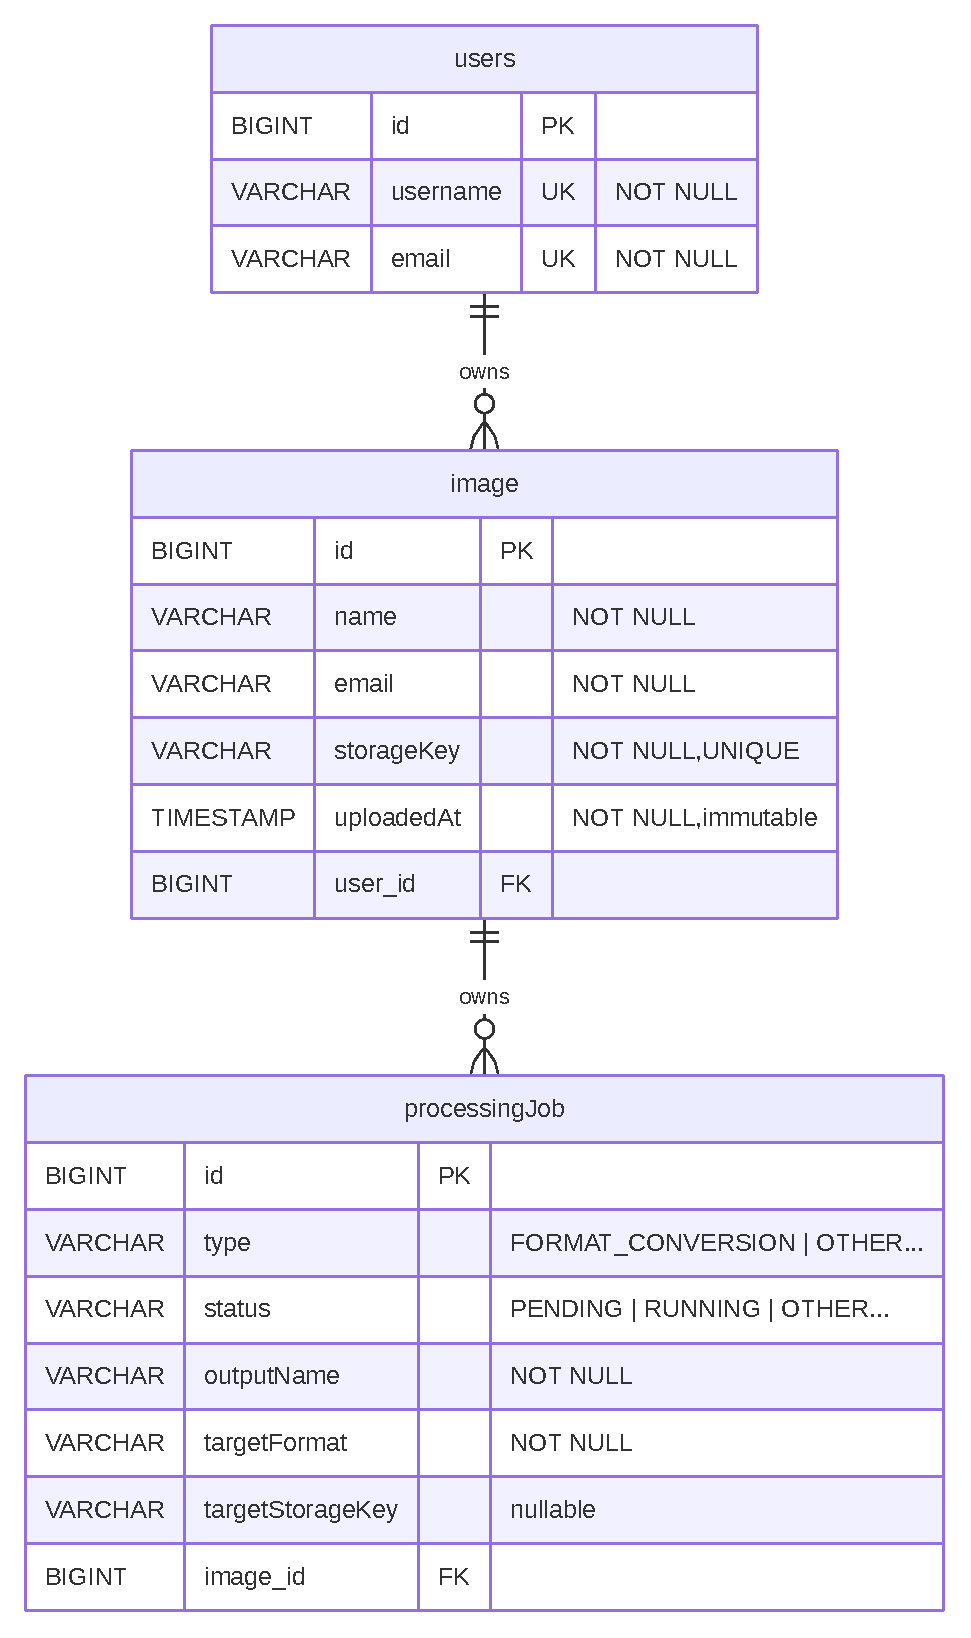
\includegraphics[width=\textwidth , height=\textheight, keepaspectratio]{images/v1-erd.pdf}
    \caption{Entity-Relationship Model showing Users, Images, and Processing Jobs.}
    \label{fig:v1-erd}
\end{figure}

\subsection{Application Structure and Development}
The monolith is organized as a single Maven project following a conventional layered package structure: \texttt{controller} (REST endpoints for users, images, and jobs), \texttt{service} (business logic and transactional boundaries), \texttt{processor} (physical I/O, isolated to \texttt{ImageProcessor}), \texttt{entity} (JPA-mapped domain classes), \texttt{repository} (Spring Data JPA interfaces), \texttt{dto} (immutable API records), \texttt{exception} (domain exceptions and the global handler), and \texttt{utils} (format validation). This structure was chosen deliberately to mirror, within a single process, the boundaries that would later become service boundaries: the \texttt{controller} package is what becomes the Gateway's public surface in \emph{v2}, while \texttt{service}, \texttt{entity}, and \texttt{repository} become the Orchestrator, and \texttt{processor} becomes the AI Worker.

The domain layer consists of three JPA entities. \texttt{User} holds \texttt{username} and \texttt{email}, both \texttt{NOT NULL UNIQUE}. \texttt{Image} holds the original \texttt{name}, a normalized \texttt{format}, a UUID-based \texttt{storageKey} used for filesystem lookup, and an immutable \texttt{uploadedAt} timestamp set via \texttt{@PrePersist}, linked to its owner through a \texttt{@ManyToOne} association. \texttt{ProcessingJob} holds a \texttt{type} and \texttt{status} enum, an \texttt{outputName}, a \texttt{targetFormat}, and a \\ nullable \texttt{targetStorageKey} populated only once execution completes, linked to its source image through a \texttt{@ManyToOne} association. Both foreign keys carry \texttt{CASCADE DELETE} semantics.

The public API surface, all under the \texttt{/api} prefix, exposes ten endpoints across the three resources: user registration and listing (\texttt{POST}/\texttt{GET /api/users}), per-user image listing and cascade-delete (\texttt{GET}/\texttt{DELETE /api/users/\{id\}/...}), image upload with magic-byte validation and job creation/listing (\texttt{POST}/\texttt{GET /api/images/...}), and job triggering, polling, result download, and deletion (\texttt{POST}/\texttt{GET}/\texttt{DELETE /api/jobs/\{id\}/...}). Every endpoint returns one of a small, consistent set of status codes (\texttt{200}, \texttt{201}, \texttt{202}, \texttt{204}, \texttt{400}, \texttt{404}, \texttt{409}, \texttt{413}, \texttt{415}, \texttt{500}), each tied to a specific, named condition rather than left as an implementation detail of the framework, for instance, \texttt{415} is raised exclusively by \texttt{ImageFormatValidator} when magic-byte inspection fails to match a supported format, independent of the file's extension or declared \texttt{Content-Type}. 

Two cross-cutting implementation choices shaped how the service layer was written, independent of any single endpoint. First, transactional boundaries are explicit rather than left at Spring's defaults: state-mutating service methods use \texttt{@Transactional} with \\ \texttt{READ\_COMMITTED} isolation, while pure-read methods are marked \texttt{readOnly = true}; the asynchronous job-execution path deliberately runs \emph{outside} any long-lived transaction, committing the \\ \texttt{targetStorageKey} assignment and final status update in a short transaction while the actual FFmpeg subprocess call executes without holding a database connection for its duration. Second, critical service and storage methods are annotated with Micrometer's \texttt{@Observed}, producing traces and metrics from the very first milestone, well before any consuming observability backend (Prometheus/Grafana, or later OpenTelemetry) was deployed, establishing the instrumentation baseline early was a deliberate choice, discussed further in Chapter \emph{Results}, Section \emph{Cross-Cutting Results}.

Development itself proceeded against a PostgreSQL instance and FFmpeg binary installed directly on the host (Arch Linux), with Spring Boot's profile mechanism \\ (\texttt{application-local.properties}, git-ignored, activated via \\ \texttt{spring.profiles.active=local}) supplying local credentials over the base \\ \texttt{application.properties}. An early implementation choice, exposing the domain model via Spring Data REST for rapid HATEOAS-style prototyping, was deliberately abandoned in favor of explicit Spring MVC controllers before the milestone was considered complete, for the reasons discussed below.

\subsection{Key Implementation Decisions}
The \texttt{ImageService}/\texttt{ImageProcessor} split was made with the following milestone explicitly in mind: the \texttt{@Async} boundary between them was designed to later become a network or message-queue boundary between an Orchestrator and a Worker service, with minimal change to the orchestration logic itself. This decision paid off directly in \emph{v2} and again in \emph{v4}, where the same dispatch logic reappears first as a synchronous HTTP call and later as a Kafka publish, in both cases without restructuring the job-lifecycle state machine. A second notable decision was rejecting Spring Data REST/HATEOAS, initially used for rapid prototyping, in favor of explicit Spring MVC controllers, decoupling the public API contract from the database schema and avoiding \texttt{LazyInitializationException} risks from open-session patterns. Even if it was discarded the Spring Data REST/HATEOAS approach was documented for educational purposes as it's part of the DevOps course topics.

\subsection{Validation}
The job lifecycle (\texttt{PENDING} $\rightarrow$ \texttt{RUNNING} $\rightarrow$ \texttt{DONE}/\texttt{FAILED}) was validated through JUnit 5 and Mockito unit/service-layer tests, with an H2 in-memory database for integration tests not requiring the full context. File format validation was tested against magic-byte detection rather than trusted file extensions.

\subsection{Critical Assessment vs. Goal}
Against the success criteria defined in Chapter \emph{Goal}, this milestone is met: the application exposes a complete REST API over the full domain model, and an end-to-end job (upload $\rightarrow$ process $\rightarrow$ download) completes and is automatically testable. The deliberate anticipation of the future service boundary in the \texttt{ImageService}/\texttt{ImageProcessor} split is, in retrospect, the single decision from this milestone with the largest downstream payoff.

\section{Microservices}

\subsection{Architecture}
The monolith was decomposed into three services along the boundary anticipated in \emph{v1}: a \textbf{Gateway} (public API, BFF pattern, UI serving), an \textbf{Orchestrator} (domain logic, JPA entities, job lifecycle, owns PostgreSQL), and a Python \textbf{AI Worker} (FastAPI, FFmpeg, rembg, Deformable DETR). A shared \texttt{common} module carries DTOs, enums, and exceptions between the two Java services, deliberately kept free of Spring dependencies to avoid transitive bean-registration conflicts. Figure~\ref{fig:v2-architecture} shows the resulting traffic flow.

% figure: v2 architecture flowchart (sprint-2-microservices-recap.md §1, mermaid flowchart)
\begin{figure}[htbp]
    \centering
    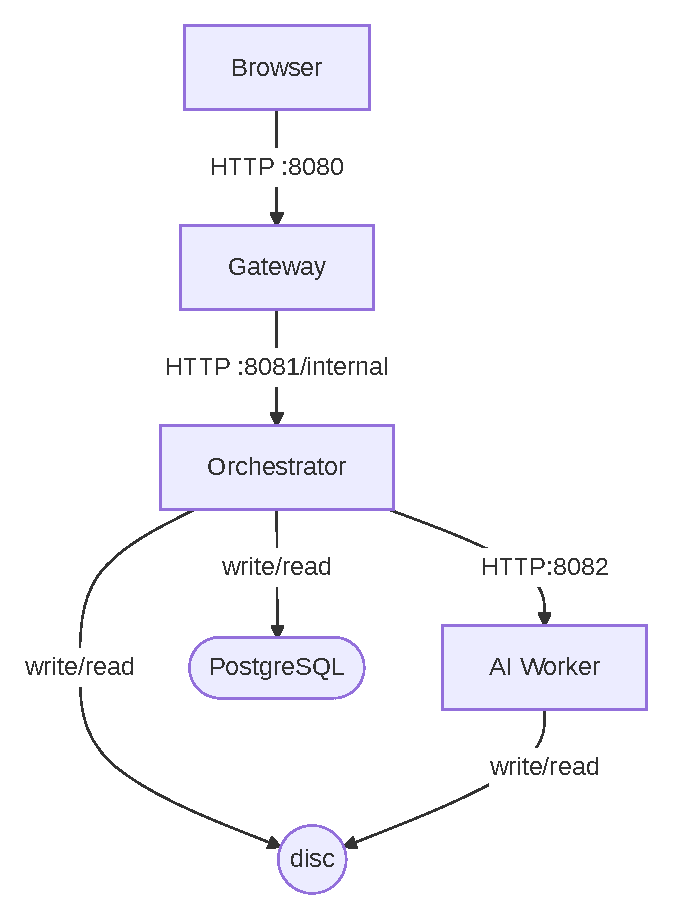
\includegraphics[width=\textwidth , height=\textheight, keepaspectratio]{images/v2-architecture.pdf}
    \caption{Architecture flowchart (v2): microservices decomposition: Java Orchestrator and Gateway, Python Worker, PostgreSQL}
    \label{fig:v2-architecture}
\end{figure}

\subsection{Application Structure and Development}
The single Maven project became a multi-module reactor build with a parent POM at the repository root (packaging \texttt{pom}), and three Java-facing modules plus one Python project: \texttt{common} (plain JAR, no Spring dependency, shared DTOs/enums/exceptions), \texttt{orchestrator} (Spring Boot fat JAR, domain logic and JPA persistence), \texttt{gateway} (Spring Boot fat JAR, public API and UI serving), and \texttt{worker} (Python, \texttt{uv} project). Maven resolves the build order automatically from the module dependency graph; \texttt{common} builds first, since both \texttt{orchestrator} and \texttt{gateway} depend on it, so \texttt{mvn clean package} from the repository root produces all three Java artifacts in the correct order with a single command.

The \texttt{common} module carries nine DTOs (including three worker-communication records introduced specifically for this milestone: \texttt{ConvertFormatRequest}, \texttt{RemoveBackgroundRequest}, \texttt{ObjectDetectionRequest}, plus a matching \texttt{WorkerResponse}), two enums (\texttt{JobStatus}, \texttt{JobType}), and three exception classes. Its only permitted dependencies are \\ \texttt{jackson-databind} and \texttt{jakarta.validation-api}, a constraint enforced not by convention but by a concrete failure encountered during development: adding a Spring web dependency to \texttt{common} caused a \texttt{BeanDefinitionOverrideException} in the orchestrator, because it transitively pulled in \texttt{spring-boot-starter-jdbc}, which registered a second \texttt{transactionManager} bean conflicting with the JPA-registered one. The fix was to remove the offending dependency from \texttt{common} entirely, rather than work around the conflict downstream.

The orchestrator retains the \texttt{v1} domain model unchanged (\texttt{User}, \texttt{Image}, \texttt{ProcessingJob}) but its package structure now separates a \texttt{client} package (\texttt{WorkerClient}, calling the Python worker over HTTP) from the existing \texttt{controller}, \texttt{service}, \texttt{entity}, \texttt{repository}, and \texttt{mapper} packages, and exposes only an internal API under the \texttt{/internal} prefix (applied uniformly via \texttt{server.servlet.context-path} rather than per-controller). The public \texttt{/api/*} controllers from \texttt{v1} were removed from the orchestrator entirely and now live in the gateway. \texttt{ProcessingJobService.startAsyncProcessExecution} dispatches to the correct worker endpoint via an exhaustive \texttt{switch} expression on \texttt{JobType} with no \texttt{default} arm, a deliberate choice, discussed further below, that makes an unhandled job type a compile-time error rather than a silent runtime no-op.

One implementation detail encountered specifically at this stage is worth noting as a concrete example of a naming collision in Spring's bean registration: \texttt{WorkerClient}, annotated \texttt{@Component}, registers under the bean name \texttt{workerClient} (camelCase of the class name); the corresponding \texttt{@Bean} factory method in \texttt{WorkerWebClientConfig} therefore could not also be named \texttt{workerClient} without triggering a \texttt{BeanDefinitionOverrideException}, and was renamed to \texttt{workerWebClient()} to avoid the clash.

The gateway implements the Backend-For-Frontend pattern directly: it owns no database, uses a blocking-mode \texttt{WebClient} (rather than \texttt{RestTemplate}, which is in maintenance mode, and rather than genuinely reactive usage, since the gateway runs on a Tomcat, not reactive, runtime) to call the orchestrator, and validates inputs a second time at its own boundary, \texttt{@Validated} at the controller level, \texttt{@Min(0)} on path-variable IDs, and a \texttt{@Pattern} constraint restricting \texttt{targetFormat} to the five supported canonical values, before ever forwarding a request to the orchestrator, which independently re-validates the same constraints as the authoritative source of domain correctness.

The Python worker is a FastAPI application exposing four endpoints (\texttt{/health}, \\ \texttt{/convert\_format}, \texttt{/remove\_background}, \texttt{/detect\_objects}), with all machine-learning models, the \texttt{rembg} session and the Deformable DETR processor/model pair, loaded exactly once at startup inside a single, flat \texttt{lifespan} context manager, rather than per-request; the application does not report itself ready until this loading completes, which becomes directly relevant to readiness-probe configuration once the worker is deployed to Kubernetes in \emph{v4}.

\subsection{Key Implementation Decisions}
Communication between the Java services and the Python worker required reconciling Jackson's default camelCase serialization with the worker's snake\_case Pydantic models; per-field \texttt{@JsonProperty} annotations proved to be the reliable solution, after \texttt{@JsonNaming} was found unreliable on Java records. The Gateway was built as a genuine Backend-For-Frontend: it owns no database, forwards all domain requests to the Orchestrator, and re-stamps error responses so that a failure originating in the Orchestrator's internal API is transparently reported to the browser under the Gateway's public path.

\subsection{Validation}
A stateful, asynchronous end-to-end pytest suite exercises all three services under concurrency: it creates a user, uploads a mathematically valid 1x1 PNG (deliberately avoiding EXIF-related decoder edge cases), fires three job types in parallel via a thread pool, polls until completion, and performs cascade-delete cleanup.

\subsection{Critical Assessment vs. Goal}
The success criterion for this milestone, the AI worker deployable, restartable, and scalable independently of the gateway and orchestrator, with no shared process or failure domain, is met. The clean DTO contract established in the \texttt{common} module and the strict internal/public API split proved to be a stable foundation: no service boundary introduced here was revisited in later milestones.

\section{Containerization}

\subsection{Architecture}
Each service was packaged as a Docker image, with the Java services (Gateway, Orchestrator) built via a two-stage Maven/Alpine process and the Python worker built on \\ \texttt{python:3.13-slim} rather than Alpine, since musl libc is incompatible with the pre-compiled glibc wheels required by PyTorch. A Docker Compose blueprint orchestrates all four containers (including PostgreSQL) with explicit startup-ordering via health-checked \texttt{depends\_on}. Figure~\ref{fig:v3-architecture} shows the container network boundaries.

% figure: v3 architecture flowchart (sprint-2-containerization-recap.md §1, mermaid flowchart)

\begin{figure}[htbp]
    \centering
    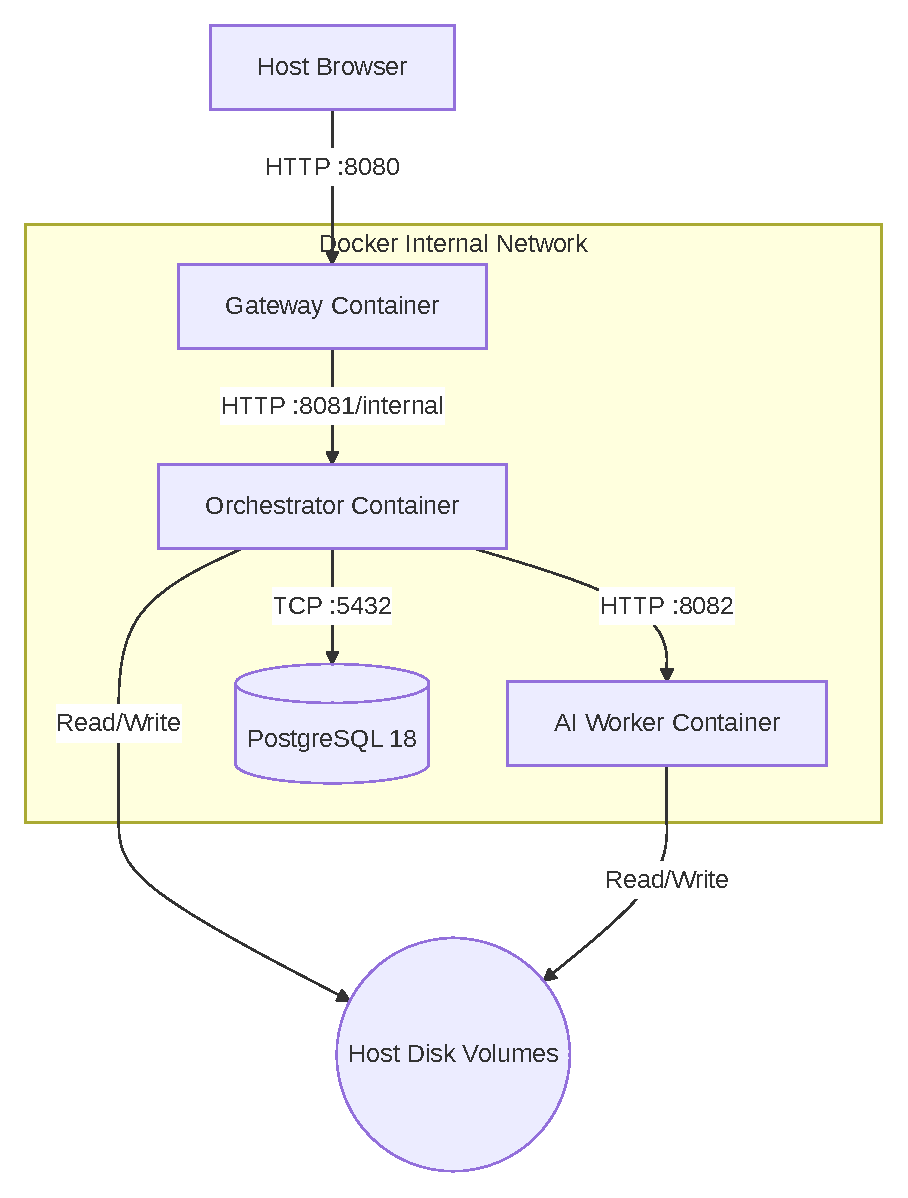
\includegraphics[width=\textwidth , height=0.85\textheight, keepaspectratio]{images/v3-architecture.pdf}
    \caption{Architecture flowchart (v3): containerizaition and orchestrationand orchestration  with Docker and Docker-Compose}
    \label{fig:v3-architecture}
\end{figure}

\subsection{Application Structure and Development}
No new services were introduced at this milestone; the existing Gateway, Orchestrator, and Worker were each packaged into a Docker image, and a fourth container (PostgreSQL) joined them under a single \texttt{docker-compose.yml}. Both Java services follow an identical two-stage Dockerfile structure: a build stage (\texttt{maven:3.9.16-eclipse-temurin-21-alpine}) that copies only the POM files and downloads Maven dependencies before the source code is copied in, so that a source-only change does not invalidate the dependency-download Docker layer, followed by a runtime stage (\texttt{alpine/java:21-jre}) that strips away the JDK, Maven, and OS build tooling entirely, running only the compiled JAR. The Python worker's Dockerfile instead uses \texttt{uv} in its build stage to sync dependencies into an isolated \texttt{.venv}, and its runtime stage installs \texttt{ffmpeg} and \texttt{curl} via \texttt{apt-get} before invoking the entrypoint directly against the copied virtual environment's interpreter (\texttt{/app/.venv/bin/python main.py}), bypassing any global Python installation in the image.

All four Spring Boot and FastAPI \texttt{application.properties}/environment-variable references to \texttt{localhost} were removed at this stage; database host, credentials, and the worker's base URL are now injected exclusively through environment variables (e.g. \\ \texttt{\${POSTGRES\_HOST:localhost}}), read by Docker Compose from a git-ignored \texttt{.env} file. \\ \texttt{docker-compose.yml} additionally encodes explicit startup ordering via \\ \texttt{depends\_on: condition: service\_healthy}: PostgreSQL's healthcheck uses \\ \texttt{pg\_isready} natively, while the worker's uses \texttt{curl} against its own \texttt{/health} endpoint with an extended \texttt{15s} interval and \texttt{10} retries, since the worker is not considered healthy until its ML models have finished loading into memory, which can take significantly longer than a typical container healthcheck window.

Development and validation at this stage relied on two custom scripts committed alongside the compose file: an infrastructure-audit Bash script and a stateful, concurrent end-to-end pytest suite reused unchanged from \emph{v2}, both discussed in \emph{Validation} below.

\subsection{Key Implementation Decisions}
All custom application containers were hardened to run as a non-root user, \texttt{appuser}, which is where the single most subtle failure mode of this milestone surfaced. Docker's default behavior, when a Compose volume mount targets a container directory that does not yet exist, is to create that directory as \texttt{root} at mount time. Because the ML model caches (\texttt{HF\_HOME}, \texttt{U2NET\_HOME}) and the shared storage directory are all volume-mounted, the non-root \texttt{appuser} attempting to download a \textasciitilde400MB \texttt{.onnx} model into a root-owned cache directory failed with a fatal \texttt{Permission Denied} error, a failure that appears identical to a networking or download problem at first inspection, and only becomes traceable to ownership once the container's effective UID is checked. The fix was to pre-create every shared data and cache directory explicitly during the image build, and \texttt{chown} them to \texttt{appuser:appgroup} before any volume is ever mounted over them:

\begin{verbatim}
RUN mkdir -p /tmp/imageprocessing/data \
             /home/appuser/.cache/huggingface \
             /home/appuser/.u2net && \
    chown -R appuser:appgroup /app /tmp/imageprocessing/data /home/appuser
\end{verbatim}

This is a good illustration of a failure mode that only appears once two independently reasonable design decisions, non-root execution and volume-persisted caches, are combined; neither one alone would have surfaced it.

\subsection{Base Image Strategy: Alpine vs. Debian Slim}
The two Java services and the Python worker deliberately use different Linux base image families, and this is a considered decision rather than an inconsistency. The Java runtime stage uses Alpine Linux specifically for its minimal image size, which Alpine achieves in part by using \texttt{musl libc} instead of \texttt{glibc}. The Python worker cannot make the same choice: heavy machine-learning dependencies (PyTorch, Torchvision) are distributed as pre-compiled \texttt{glibc} wheels, and \texttt{musl libc}'s binary incompatibility with those wheels would force them to be compiled from source inside the image build, which is both slow and fragile. The worker therefore uses \texttt{python:3.13-slim}, a Debian-based image that preserves \texttt{glibc} compatibility while remaining considerably smaller than a full Debian image. The general principle this illustrates, that a single "smallest base image" policy cannot be applied uniformly across a polyglot stack once native/compiled dependencies are involved, is treated here as a deliberate per-service decision rather than left as an unexplained inconsistency between the two Dockerfile families.

\subsection{Alternative Build Strategy: Cloud Native Buildpacks}
As a supplementary experiment, the two Java services were also built using Cloud Native Buildpacks via the \texttt{spring-boot:build-image} Maven goal, requiring no additional plugin declaration since \texttt{spring-boot-maven-plugin} was already present in both modules:

\begin{verbatim}
mvn -pl gateway      spring-boot:build-image -DskipTests
mvn -pl orchestrator spring-boot:build-image -DskipTests
\end{verbatim}

This delegates image construction to the Paketo Buildpacks provider, which auto-detects the Java 21 runtime and produces a layered OCI image without a hand-authored Dockerfile, running as non-root by default with no explicit user configuration required. The approach was evaluated and explicitly not carried forward as the project's canonical build path, for three reasons: it offers materially less transparency and control over the resulting image layers than the hand-authored multi-stage Dockerfiles; it produces larger images than the Alpine-based runtime stage used in Section \emph{Base Image Strategy}; and, most decisively, Paketo's Java buildpack does not cover Python runtimes at all, so the Worker's \texttt{glibc}/PyTorch constraints would have mandated a hand-authored Dockerfile regardless, at which point maintaining two different build philosophies for three services offered no net simplification. The experiment is documented here as a considered and rejected alternative, consistent with the stakeholder-review pattern described in Chapter \emph{Approach}, rather than omitted as if it had not been evaluated.

\subsection{Validation}
An automated Bash script (\texttt{validate\_infra.sh}) audits the running cluster against the hardening constraints: container health, network isolation (internal ports not exposed to the host), correct Gateway exposure, execution as \texttt{appuser}, and internal DNS resolution between containers. The \emph{v2} end-to-end pytest suite was re-run unchanged against the containerized stack, confirming behavioral parity between the bare-process and containerized deployments.

\subsection{Critical Assessment vs. Goal}
Both success criteria, non-root execution for every service, and a full stack startup from a single command with no manual host dependency installation, are met and independently validated by \texttt{validate\_infra.sh}. An alternative build strategy (Cloud Native Buildpacks) was evaluated for the Java services and explicitly not carried forward, in favor of the hand-authored Dockerfiles' smaller image size and finer-grained control, as discussed in Chapter \emph{Approach}.

\section{Kubernetes}

\subsection{Architecture}
The containerized stack was deployed onto a Minikube cluster as five workloads: \texttt{gateway}, \texttt{orchestrator}, and \texttt{worker} as Deployments, and \texttt{postgres} and \texttt{kafka} as StatefulSets, fronted by an NGINX Ingress Controller. Synchronous HTTP communication between the Orchestrator and Worker was replaced with two Kafka topics (\texttt{job.requests}, \texttt{job.results}), and a KEDA \texttt{ScaledObject} scales the Worker between 1 and 10 replicas based on consumer lag. Figure~\ref{fig:v4-architecture} shows the full deployment topology.

% figure: v4 architecture flowchart (sprint-3-recap.md §1, mermaid flowchart)

\begin{figure}[htbp]
    \centering
    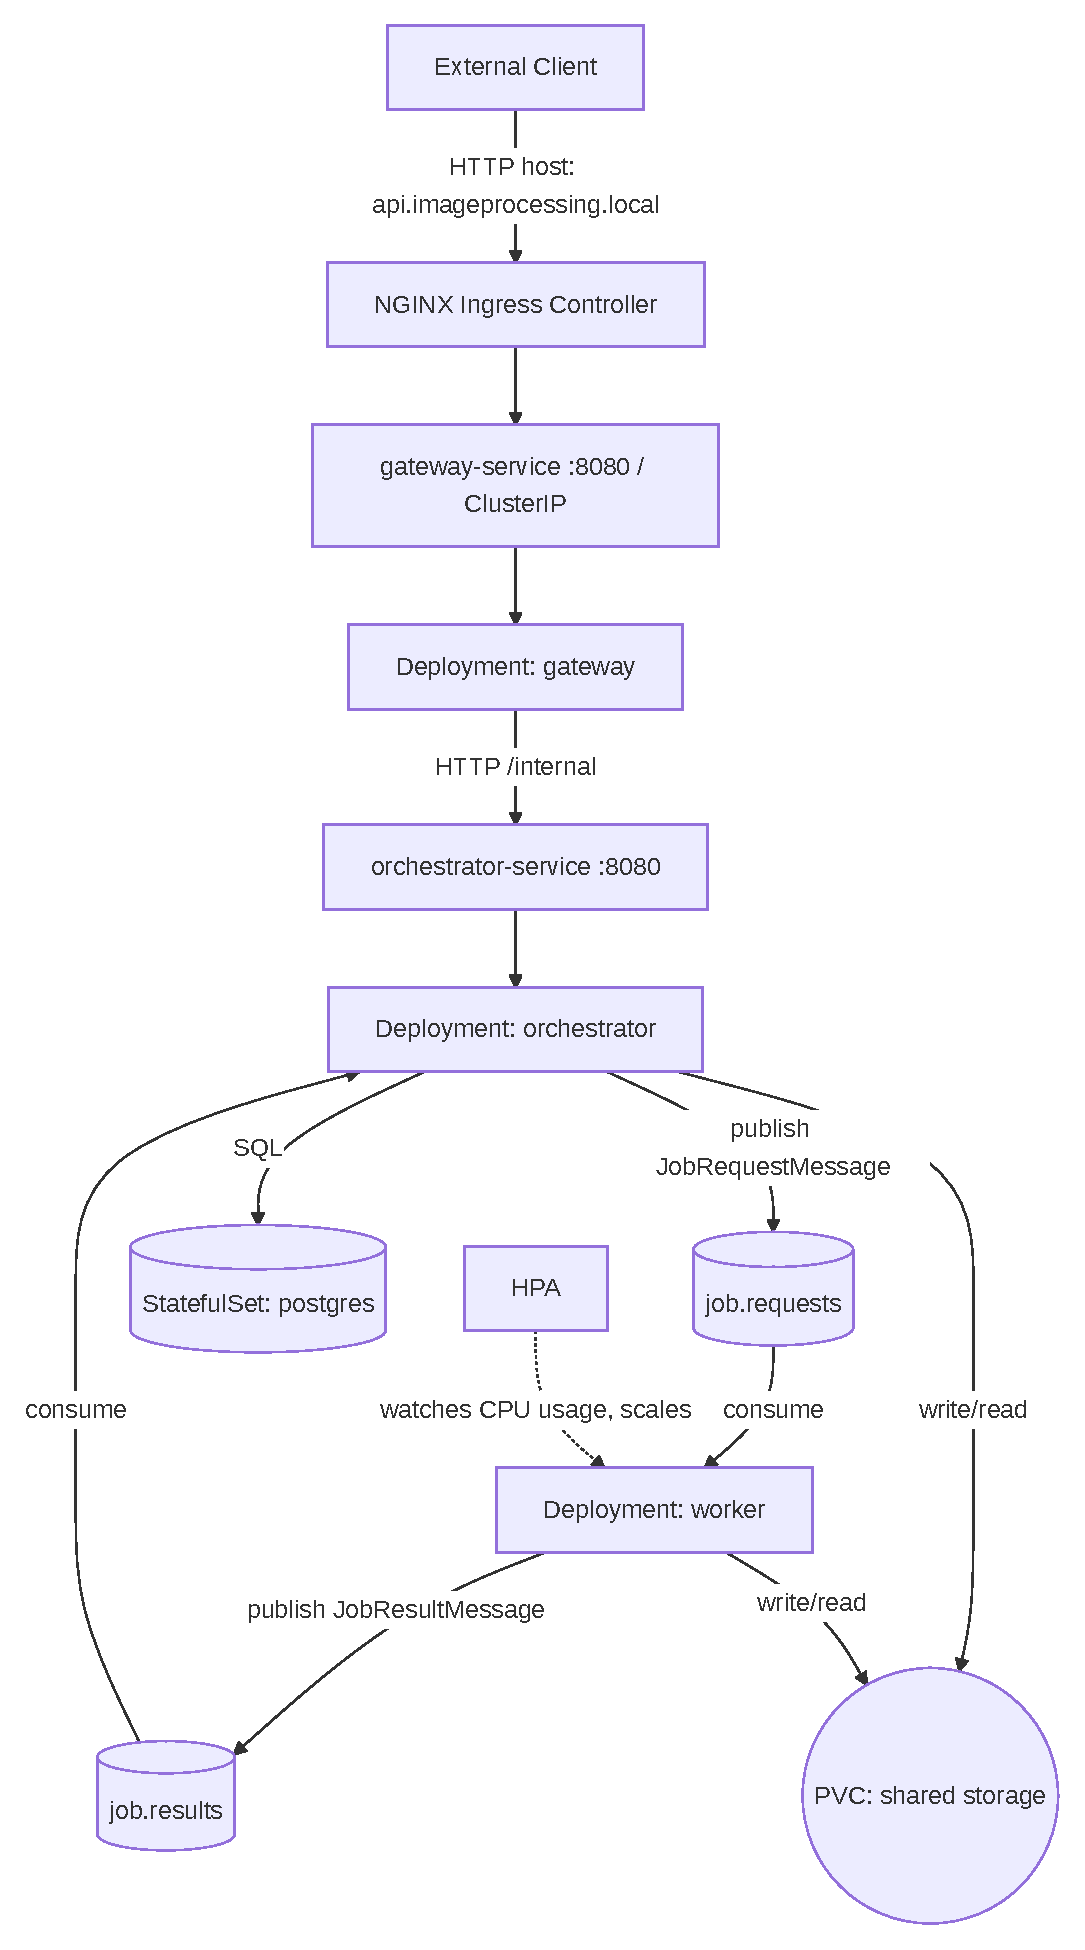
\includegraphics[width=\textwidth , height=0.85\textheight, keepaspectratio]{images/v4-architecture.pdf}
    \caption{Architecture flowchart (v4): local Minikube, Deployments, Ingress, Stateful Sets, PVs and PVCs}
    \label{fig:v4-architecture}
\end{figure}

\subsection{Application Structure and Development}
The containerized stack was deployed onto a single-node Minikube cluster, with all Kubernetes manifests organized under a top-level \texttt{k8s/} directory, one subdirectory per component (\texttt{gateway/}, \texttt{orchestrator/}, \texttt{worker/}, \texttt{postgres/}, \texttt{kafka/}, plus a shared \texttt{storage/}). Every resource is scoped to a dedicated \texttt{imageprocessing} namespace, isolating the application from the cluster's \texttt{default} namespace and from any other workload. Because Minikube runs its own isolated Docker daemon, application images had to be built against that daemon specifically (\texttt{eval \$(minikube docker-env)}) rather than the host's, with third-party images such as \texttt{postgres:18-alpine} loaded in explicitly via \texttt{minikube image load} to avoid an unnecessary re-pull.\footnote{The Gateway service is deployed under the resource name \texttt{frontend} (\texttt{frontend-service}, \texttt{frontend-config}, \texttt{frontend-ingress}), a naming inconsistency inherited from the fact that the \texttt{gateway/} source directory was never renamed even though its published image and Kubernetes resources were; the underlying service is the same Gateway/BFF discussed throughout this report.}

\subsection{Progressive Deployment Maturity: The Three-Lecture Evolution}
Rather than presenting Kubernetes deployment as a single, final configuration, the deployment procedure was deliberately built and documented in three progressively more mature stages, mirroring how the course itself introduces Kubernetes concepts incrementally. All three configurations remain functional and independently deployable; each corresponds to a distinct point in the course's own DNS/configuration maturity curve, and each demonstrates a specific class of Kubernetes primitive. Crucially, the three lecture configurations are simpler than, and distinct from, the final architecture described in the remainder of this chapter: none of them include Kafka or KEDA, which are introduced only once past this progression, on top of the third and most mature lecture configuration.
\subsubsection{Lecture one}
The first stage deploys only bare \texttt{Pod} manifests to the \texttt{default} namespace, with \\ \texttt{imagePullPolicy: Never}, since no image is pushed to a registry at this point. No \texttt{Service} objects exist yet, so pods have no stable DNS entry; every downstream configuration value that depends on another pod's address (the Orchestrator's database host, the Worker's URL) must be hand-patched with the IP address retrieved via \texttt{kubectl get pod -o wide} after each pod starts, and the deployment order is strictly manual: PostgreSQL first, then the Orchestrator and Worker, then the frontend. Bare pods carry no self-healing: if the Kubernetes out-of-memory killer or a node failure terminates a pod, it does not come back on its own.
\subsubsection{Lecture two}
The second stage introduces the \texttt{imageprocessing} namespace together with Kubernetes \texttt{Secret} and \texttt{ConfigMap} objects and \texttt{PersistentVolume}/\texttt{PersistentVolumeClaim} storage, while still deploying bare pods. This is the point at which credentials and environment-specific configuration stop being hardcoded into pod specs, and at which the ML model caches and shared processing storage first survive a pod restart rather than being re-downloaded or lost every time. DNS still has no Service-based solution at this stage; every cross-pod reference still requires the same manual IP-retrieval-and-patch cycle as the first stage. Architecturally, this stage's contribution is entirely about the durability and confidentiality of state, not about networking.
\subsubsection{Lecture three}
The third stage introduces \texttt{Service} objects (\texttt{ClusterIP} for internal components), converts the bare pods to \texttt{Deployment} and \texttt{StatefulSet} controllers, adds a plain CPU-based \texttt{HorizontalPodAutoscaler} on the Worker (1--5 replicas, targeting 70\% average CPU utilization), and adds an NGINX \texttt{Ingress} for external access. This is the point at which manual IP propagation disappears entirely: every cross-component reference resolves through Kubernetes' internal DNS by Service name, external access moves from a privileged \texttt{port-forward} tunnel to a proper host-based Ingress route, and, because workloads are now managed by controllers rather than bare pods, a crashed or deleted pod is automatically recreated without any manual reapplication. Security posture improves alongside resilience at this stage for a structural reason, not an incidental one: with Services in place, \texttt{ClusterIP} can be used to keep every internal component (PostgreSQL, Orchestrator, Worker) unreachable from outside the cluster network by construction, leaving the Ingress-fronted Gateway as the only intentionally exposed surface, a guarantee that bare pods, with no Service-level access control at all, cannot express. Probe timing at this stage is summarized in Table~\ref{tab:v4-probes}.

\begin{table}[h]
\centering
\begin{tabular}{|p{4.0cm}|p{5.5cm}|p{2.0cm}|p{1.5cm}|}
\hline
\textbf{Service} & \textbf{Mechanism} & \textbf{Readiness delay} & \textbf{Liveness delay} \\
\hline
Frontend (Gateway) & httpGet \texttt{/actuator/health} & 5s & 20s \\
\hline
Orchestrator & httpGet \texttt{/internal/actuator/health} & 5s & 15s \\
\hline
Worker & httpGet \texttt{/health} (+ startup probe, up to 10min) & 0s\textsuperscript{*} & 0s\textsuperscript{*} \\
\hline
Postgres & exec \texttt{pg\_isready} & 10s & 60s \\
\hline
\end{tabular}
\caption{Probe timing at the v4 (Kubernetes) milestone, lecture-3 baseline configuration. \textsuperscript{*}Worker readiness/liveness delays are measured from startup-probe success, not pod start, due to the dedicated \texttt{startupProbe} gating model loading.}
\label{tab:v4-probes}
\end{table}

This third stage is deliberately the last point at which the deployment is simple enough to present as a self-contained classroom walkthrough; the remainder of this chapter describes what was built on top of it: Kafka-mediated asynchronous processing. The CPU-based HPA was retained as the primary scaling mechanism for the final deployment to align with course objectives, while Kafka-lag-driven autoscaling via KEDA was tested as a collateral experiment.

\subsection{Workload Patterns: Deployments, StatefulSets, and Init Containers}
Kubernetes schedules all pods in a cluster concurrently, unlike Docker Compose's ordered \texttt{depends\_on: condition: service\_healthy}. This surfaced directly as a startup race: the Orchestrator would attempt to open a database connection pool before PostgreSQL had finished initializing, producing crash loops on first deploy. Increasing the liveness probe's \texttt{initialDelaySeconds} alone (from a default value to a temporary 60 seconds) prevented Kubernetes from prematurely killing the pod during this window, but did not eliminate the underlying crash-loop behavior, since it addressed the symptom rather than the ordering problem itself.

The definitive fix was an \texttt{initContainer} pattern: a lightweight \texttt{wait-for-postgres} container, using the \texttt{postgres:18-alpine} image purely for its native client tools, runs a \texttt{pg\_isready} polling loop every two seconds ahead of the Orchestrator's main container. Init containers run sequentially before the main container starts and are restarted on failure by Kubernetes itself, holding the pod in \texttt{PodInitializing} until they succeed. With this in place, the Orchestrator's main-container liveness delay could be safely reduced back to 15 seconds, since the concurrent-startup race is now absorbed entirely by the init container rather than papered over with a longer timeout.

Stateless services (\texttt{gateway}, \texttt{orchestrator}, \texttt{worker}) were converted from bare pods to \texttt{Deployment} controllers, carrying their environment variables, \texttt{envFrom} references, and volume mounts across unchanged from the original pod specs. PostgreSQL and Kafka, in contrast, required \texttt{StatefulSet} controllers rather than Deployments, since both need guarantees a Deployment does not provide: a stable, predictable pod DNS name (\texttt{postgres-0}, \texttt{kafka-0}, rather than a Deployment's randomly-suffixed pod names), and, via \\ \texttt{volumeClaimTemplates}, an automatically provisioned and consistently re-bound PersistentVolumeClaim per replica, so that a restarted \texttt{postgres-0} reattaches to the exact same volume rather than a fresh, empty one.

Probe configuration was tuned per service according to how long each takes to genuinely become ready. The most significant divergence is the Worker: its startup probe allows up to ten minutes for the machine-learning models to load (\texttt{failureThreshold: 120} at a five-second period) before readiness and liveness probes even begin evaluating, accommodating the loading time established already in \emph{v2}'s \texttt{lifespan} startup behavior, a direct example of an application-level design decision from an earlier milestone dictating an infrastructure-level configuration value two milestones later.

\subsection{Kafka Message Contracts and Delivery Semantics}
Building on the lecture-3 configuration described above, synchronous HTTP communication between the Orchestrator and Worker, in place since \emph{v2}, was replaced with two Kafka topics: \texttt{job.requests} (Orchestrator $\to$ Worker) and \texttt{job.results} (Worker $\to$ Orchestrator). This choice deliberately mirrors a constraint already present in the Orchestrator's code: the exhaustive \texttt{switch} on \texttt{JobType} introduced in \emph{v2}, which has no \texttt{default} arm and therefore forces a compile-time decision whenever a new job type is added. The two-topic design preserves that same property at the infrastructure level; adding a job type becomes a new dispatch-table entry, not new topic provisioning or new consumer subscriptions. Both topics are keyed by \texttt{jobId}, guaranteeing that every message belonging to a given job is processed in order by a single consumer.

Message ownership of the output storage key was a design point revisited mid-implementation. The original rule, established in \emph{v1}, is that \texttt{targetStorageKey} is generated by \\ \texttt{ProcessingJobService.processJob()} before any processing begins. An early draft of the Kafka integration broke this rule by instead assigning the key from the Worker's result message upon completion. This was reverted back to creation-time assignment once its consequences under Kafka's delivery model were examined, since completion-time assignment is not idempotent under message redelivery (a reprocessed message could regenerate a different key and orphan a partially-written file). Creation-time assignment guarantees the same key on every retry and keeps \texttt{GET /api/jobs/\{id\}} accurate the instant a job transitions to \texttt{RUNNING}, rather than only once the Worker eventually replies.

Delivery semantics are deliberately at-least-once rather than exactly-once, since exactly-once would require transactional producers and consumers on both the JVM and Python sides, judged disproportionate for a single-broker, thesis-scale deployment. This is handled explicitly rather than left as an unhandled edge case: the Worker's consumer commits its Kafka offset only after successfully publishing to \texttt{job.results}, so a crash mid-inference causes the same request to be redelivered rather than silently dropped. The Orchestrator's result listener is idempotent by construction, since re-applying the same \texttt{DONE}/\texttt{FAILED} status twice has no observable effect. One gap is documented rather than silently accepted: if the Orchestrator's own publish call fails outright (e.g. the broker is unreachable), the job is flipped directly to \texttt{FAILED} with no retry; a transactional outbox pattern would close this gap but was judged out of scope for this project's scale.

Kafka itself runs as a single-broker, KRaft-mode \texttt{StatefulSet} \\ (\texttt{apache/kafka:3.9.0}, \texttt{process.roles=broker,controller}), deliberately avoiding a separate Zookeeper component. Topic auto-creation is disabled in the cluster deployment; both topics are instead created explicitly by a one-shot Kubernetes \texttt{Job}, with a fixed, deliberately chosen partition count: 10 for \texttt{job.requests}, 3 for \texttt{job.results}, rather than whichever count the first producer happened to trigger. 

\subsection{Autoscaling Approaches: KEDA vs. HPA}
The partition count of 10 for \texttt{job.requests} established above is not incidental: it directly dictates the scaling ceiling for the Worker. Because Kafka assigns at most one partition per consumer within a consumer group, a Worker scaled beyond 10 replicas would receive no partitions and sit fully idle. 

Once the asynchronous queueing mechanism was in place, the autoscaling strategy was evaluated. From a strictly architectural standpoint, as discussed in Chapter \emph{State of the Art}, event-driven scaling using KEDA (scaling directly on Kafka consumer lag) is the superior approach for this workload. CPU utilization is a poor and often lagging proxy for queue backlog, especially for AI inference workers where processing time and hardware utilization (like I/O blocks) do not scale linearly with incoming HTTP requests. 

To validate this, an experimental branch successfully utilized a KEDA \texttt{ScaledObject} to scale the Worker directly on the \texttt{job.requests} consumer lag. The configuration was capped at exactly \texttt{maxReplicaCount: 10} to match the partition count one-to-one, with \texttt{minReplicaCount: 1} kept to avoid a scale-from-zero cold start against the Worker's lengthy model-loading window, and a \texttt{lagThreshold} of 10 messages per additional replica.

However, a deliberate compromise was made for the final deployment. Due to course constraints and the need to align with the pedagogical curriculum (which covers Kubernetes' native Horizontal Pod Autoscaler (HPA) but not third-party event-driven scalers) the main deployment relies on standard HPA. To trigger this natively, the Worker container was configured with specific CPU requests, using the CPU spikes caused by continuous Kafka polling and processing to drive scale-out events. The KEDA implementation remains documented and validated as the architecturally correct choice for this workload, while HPA serves the formal educational requirement.

\subsection{Key Implementation Decisions}
Beyond the workload, messaging, and scaling decisions discussed in the preceding subsections, one further storage-related decision is worth documenting explicitly. The shared storage \texttt{PersistentVolume}, backed by a \texttt{hostPath} on the Minikube node, initially declared \texttt{ReadWriteMany} to reflect its intended use (both the Orchestrator and the Worker write to it). This was corrected mid-sprint to \texttt{ReadWriteOnce}: Kubernetes accepts the \texttt{hostPath}/\texttt{ReadWriteMany} combination syntactically, but \texttt{hostPath} has no attach/detach mechanism for the kubelet to enforce access modes against, so the declared mode was decorative rather than a real guarantee. Two Worker replicas scheduled to the same node appeared to share the volume correctly, while a replica scheduled to a different node silently received an empty, disconnected local path instead. Relabeling the volume as \texttt{ReadWriteOnce} does not fix the underlying multi-node risk; it only makes the manifest state a guarantee it can actually keep. The real constraint, that the cluster remains single-node until this migrates to a genuine \texttt{ReadWriteMany} backend such as NFS or a cloud file share, is enforced operationally rather than declaratively, and is tracked as an open follow-up in Section \emph{Cross-Cutting Results}.

\subsection{Validation}
Autoscaling was validated in two stages. First, a synthetic load test published 30 messages directly onto \texttt{job.requests}, bypassing the Orchestrator entirely so that the KEDA/Kafka trigger could be isolated from the rest of the request path; against a \texttt{lagThreshold} of 10, this is expected to drive the Worker toward $\lceil 30/10 \rceil = 3$ replicas. Second, a k6 script (\texttt{test/loadtest.js}) exercises the full public path (Ingress $\rightarrow$ Gateway $\rightarrow$ Orchestrator $\rightarrow$ Kafka $\rightarrow$ Worker) under a sustained, ramped load profile: virtual users ramp from 0 to 5 over 30 seconds, hold at 5 for three minutes, then ramp back to 0 over 30 seconds, with each user sleeping one second between iterations. The script's \texttt{setup()} phase creates a single load-test user and uploads one fixed image, so that the ramp-up exercises job creation and triggering under concurrency rather than conflating that signal with user/image creation churn; its \texttt{teardown()} phase deletes the load-test user, relying on the existing cascade-delete chain to clean up every job created during the run in a single call.

\subsection{Critical Assessment vs. Goal}
The criteria for this milestone are largely met: the system survives pod deletion without manual intervention, and the Worker scales automatically on CPU load via HPA, as demonstrated by the load tests. One caveat, carried forward honestly rather than glossed over: whether all 10 Worker replicas are actually schedulable on the single-node Minikube cluster was not validated against hard resource ceilings. 

\section{Keycloak/Auth}

\subsection{Architecture}
Keycloak was deployed within the cluster, backed by the existing PostgreSQL StatefulSet, with realm and client configuration automated via a mounted ConfigMap. The Gateway was extended into a full OAuth2/OIDC Backend-For-Frontend: it performs the Authorization Code flow, retains tokens server-side, and issues an HTTP-only session cookie to the browser, which contains no OAuth2 logic itself. Alongside this, a GitLab CI/CD pipeline was built to automatically test, build, and deploy the system. Figure~\ref{fig:v5-architecture} shows the full architecture including the authentication backchannel and CI/CD delivery path.

% figure: v5 architecture flowchart (sprint-4-part-2-keycloak-recap.md §1, mermaid flowchart)

\begin{figure}[htbp]
    \centering
    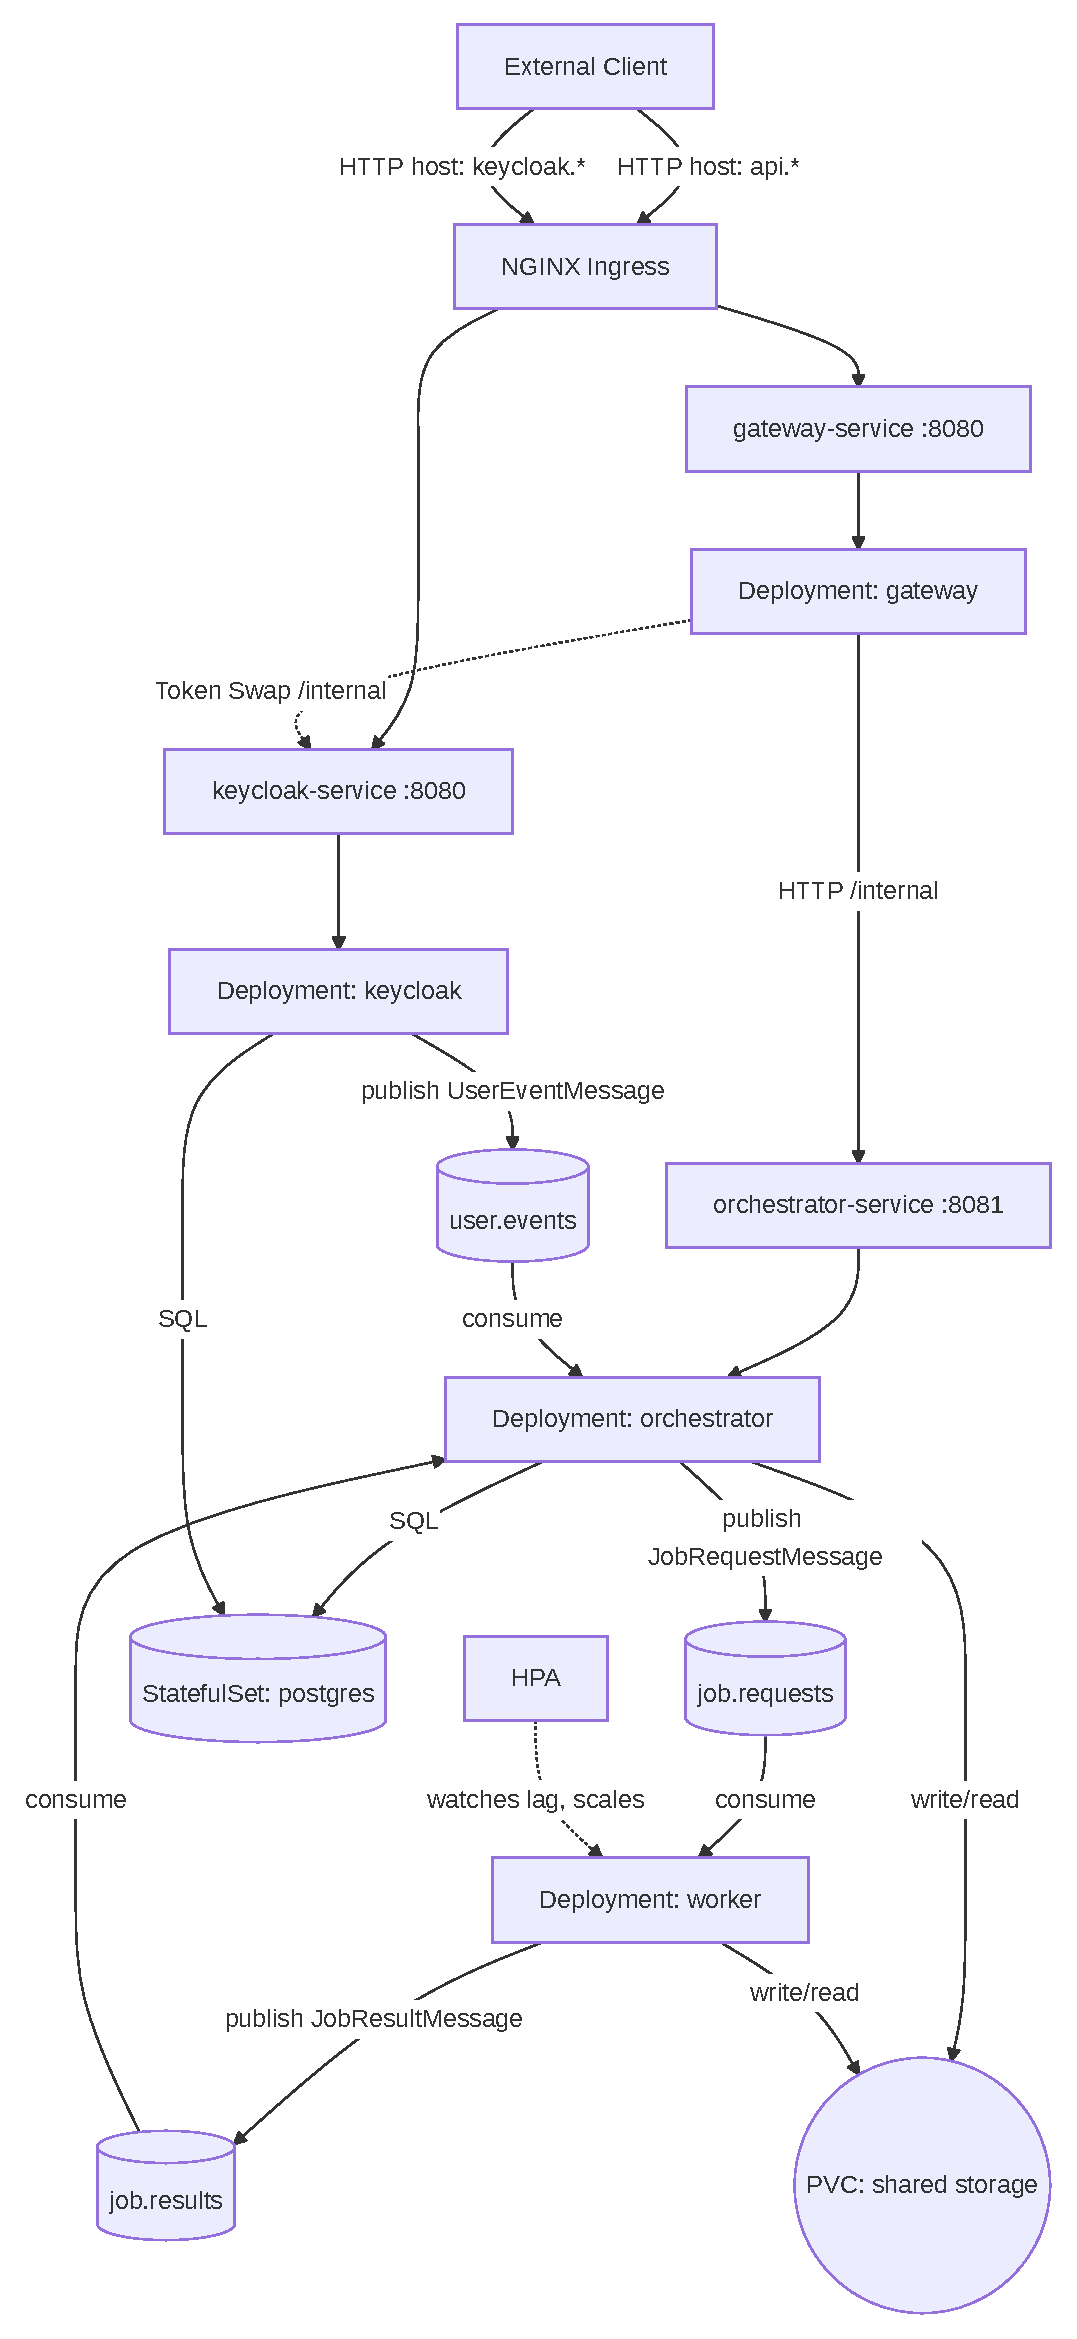
\includegraphics[width=\textwidth , height=0.85\textheight, keepaspectratio]{images/v5-architecture.pdf}
    \caption{Architecture flowchart (v5): Keycloak integration}
    \label{fig:v5-architecture}
\end{figure}

\subsection{Application Structure and Development}
Keycloak was deployed as a stateless \texttt{Deployment}, distinct from the StatefulSet pattern used for PostgreSQL and Kafka, since Keycloak itself holds no local state, all persistent state lives in its backing PostgreSQL database, provisioned by a dedicated, idempotent \texttt{keycloak-create-db} Job that creates the \texttt{keycloak} database and owner role using \\ \texttt{pg\_isready}/\texttt{psql} scripting, safe to re-run without side effects. As with the Orchestrator in \emph{v4}, an \texttt{initContainer} blocks the Keycloak pod from starting until PostgreSQL is confirmed reachable, reusing the same pattern rather than introducing a new one. Realm and client configuration (realm \texttt{imageprocessing}, client \texttt{gateway}, configured for the \\ \texttt{authorization\_code} flow with \texttt{publicClient: false} and client-secret authentication) is injected automatically on first boot via a realm-import JSON file mounted from a ConfigMap, rather than configured by hand through the admin console after deployment.

On the Gateway side, the module gained a \\ \texttt{spring-boot-starter-oauth2-client}/\texttt{spring-boot-starter-security} dependency pair and a \texttt{SecurityConfig} class securing every route except \texttt{/actuator/health} behind \\ \texttt{.oauth2Login()}. A new \texttt{MeController} bridges the two identity domains: on \texttt{GET /api/me}, it extracts \texttt{preferred\_username} and \texttt{email} from the authenticated \texttt{OidcUser} principal and calls the Orchestrator's \texttt{POST /users/find-or-create} endpoint, the synchronous path responsible for account creation discussed further below. A custom \texttt{LogoutSuccessHandler} replaces Spring's default OIDC logout handling entirely, since Keycloak enforces RP-initiated logout strictly: the handler explicitly constructs the redirect URI carrying \\ \texttt{post\_logout\_redirect\_uri} and \texttt{id\_token\_hint}, both required for Keycloak to accept the logout request rather than silently ignoring it.

\subsection{Identity Bridging and Event-Driven User Lifecycle}

\subsubsection{Keycloak as Single Source of Truth: The Event Bridge}
Keeping Keycloak authoritative over user identity and lifecycle, rather than letting the Orchestrator's database silently become a second, potentially divergent source of truth, required solving a gap that Keycloak does not close natively: out of the box, Keycloak has no mechanism to notify external systems when a user is deleted. Left unaddressed, this would have forced a choice between two designs this project explicitly rejects: either the Orchestrator polling Keycloak for changes, or account deletion being modeled as two independent, non-atomic operations performed by an administrator by hand.

The solution is \texttt{keycloak-kafka-extension}, a custom Keycloak Event Listener SPI (Service Provider Interface) plugin, built in Java 21 against Keycloak 26.0.7's extension API and packaged as a shaded "fat" JAR (via \texttt{maven-assembly-plugin}) bundling the Kafka client library (\texttt{kafka-clients} 3.7.0) directly into the artifact, since Keycloak's runtime classpath does not otherwise provide one. The extension is deployed by extending the official Keycloak image in a custom multi-stage Dockerfile: the fat JAR is copied into \texttt{/opt/keycloak/providers/}, after which \texttt{kc.sh build} bakes the extension into an optimized runtime image at build time rather than loading it dynamically at startup. The Kafka bootstrap servers and target topic are configured via environment variables \\(\texttt{KAFKA\_BOOTSTRAP\_SERVERS}, \texttt{KAFKA\_USER\_EVENTS\_TOPIC}), consistent with the externalized-configuration convention followed throughout the rest of the system.

The listener is deliberately narrow in scope: it fires exclusively on account deletion, from both possible origins Keycloak exposes, a user deleting their own account \\ (\texttt{EventType.DELETE\_ACCOUNT}) and an administrator deleting a user from the console (an \texttt{AdminEvent} with \texttt{ResourceType.USER} and \texttt{OperationType.DELETE}), and publishes a minimal JSON payload (\texttt{\{"username": "\%s", "action": "DELETE"\}}) to the \texttt{user.events} topic, keyed by username, using Keycloak's standard \texttt{StringSerializer} for both key and value. It does not listen for account creation or profile updates.

This asymmetry is intentional, not an oversight. Account creation is handled through a different, synchronous path entirely: the Gateway's \texttt{POST /users/find-or-create} call to the Orchestrator, made on a user's first successful login. Creation can be synchronous precisely because it happens on the request path of an action the user is already waiting on (logging in); deletion, in contrast, can be triggered entirely outside any request the Orchestrator is party to, most notably, by an administrator acting directly in the Keycloak console, with no Gateway or Orchestrator call involved at all. The event bridge exists specifically to close that gap, and only that gap: it is scoped to the one class of change Keycloak cannot otherwise surface to the rest of the system, rather than generalized into a full user-lifecycle event stream that would have duplicated logic already covered by the synchronous creation path.

On the consuming side, the Orchestrator implements a \texttt{UserEventListener}, \texttt{@KafkaListener}-annotated on the \texttt{user.events} topic, which invokes \texttt{userService.deleteByUsername()} on receipt, triggering the same JPA cascade-delete already used elsewhere in the domain model to remove the user's images, jobs, and physical storage files in one operation.

\subsubsection{Authentication Flow Design}
Account provisioning and self-service account management are deliberately kept separate in this system. New user accounts are created exclusively through the Keycloak administration console, by an administrator; end users cannot self-register. Once an account exists, users authenticate through the standard OIDC Authorization Code flow (Section \emph{Architecture}) and can self-manage their own profile, most notably changing their own password, through Keycloak's account management interface, without any administrator involvement for that class of action.

This split reflects a deliberate scope decision rather than an oversight: self-registration introduces a class of concerns, e-mail verification, spam and abuse prevention, account-recovery flows, that are orthogonal to the DevOps focus of this thesis and would have added implementation surface without deepening the demonstration of any architectural concept in scope. Restricting account creation to the admin console keeps Keycloak's role unambiguous: it is the authoritative source for \emph{who is allowed to exist} in the system, while remaining agnostic to how or why an account was provisioned. Combined with the event bridge described above, this gives the system a coherent, end-to-end account lifecycle story: an administrator provisions an account in Keycloak; the account is lazily mirrored into the Orchestrator's domain data on first login; the user self-manages their credentials thereafter without touching the Orchestrator at all; and if the account is ever deleted, from either side of the console, the deletion propagates back to the Orchestrator through the same event mechanism, without any path existing for the two systems' records to drift apart silently.

\subsection{Frontend and Session Security}
The frontend remains, deliberately, a static HTML/JavaScript application with no build step, templating engine, or client-side OAuth2 library, all authentication state is owned by the Gateway, and the frontend's only awareness of the session is the browser-managed, HTTP-only cookie it never directly reads. This has one direct security consequence that had to be addressed explicitly: without a templating engine to inject a per-request CSRF token into forms, Spring Security's default CSRF protection was disabled (\texttt{.csrf(csrf -> csrf.disable())}) rather than worked around with client-side token plumbing that the static frontend has no natural place to hold. This is documented here as a stated tradeoff rather than an omission, consistent with how other security-relevant simplifications in this project (e.g. \texttt{sslRequired: none} on the internal Keycloak-to-Gateway traffic, discussed in Chapter \emph{Approach}) are treated: acceptable for a thesis-scale, single-deployment-target system, and explicitly not a pattern to be carried into a multi-origin or production deployment without revisiting it.

A second frontend-facing issue surfaced once the Gateway began intercepting unauthenticated requests with a \texttt{302} redirect to the Keycloak login page: the frontend's \texttt{fetch()} calls would silently follow the redirect and then fail attempting to parse the resulting HTML login page as JSON, producing a confusing client-side error with no indication that the real cause was an expired session. The fix was made explicit in \texttt{script.js}: \texttt{loadCurrentUser()} and \texttt{refreshImagesAndJobs()} both inspect the response's \texttt{Content-Type} header, and if \texttt{text/html} is detected where JSON was expected, the frontend treats this as an authoritative signal of an expired or missing session and redirects the browser to \texttt{/}, cleanly re-triggering the login flow rather than surfacing a parse error to the user.

\subsection{CI/CD Pipeline: Build, Test, and Deploy Stages}
The GitLab CI/CD pipeline is organized into three stages, test, build, deploy, executed against the institutional \texttt{gitlab-edu.supsi.ch} instance.

\subsubsection{Test}
The \textbf{test} stage runs two independent jobs. \texttt{java-tests} executes the JUnit 5 suite for the Orchestrator and Gateway via Maven, with the \texttt{.m2} repository cached between runs to avoid re-downloading dependencies on every pipeline execution, and JaCoCo coverage parsed directly into GitLab's UI via a regular expression matched against the coverage report output. \texttt{python-tests} executes \texttt{pytest} against the Worker with \texttt{pytest-cov} producing a Cobertura-format report for coverage parity with the Java side; because the heavy ML models and FFmpeg subprocess calls are fully mocked (\texttt{monkeypatch.setitem}, \texttt{MagicMock}), this job runs without downloading any model weights, keeping it fast regardless of pipeline frequency. A third job, \texttt{integration-tests}, is intended to run Testcontainers-based database integration tests, but is marked \texttt{allow\_failure: true}: the institutional runners do not expose a Docker socket, so Testcontainers cannot start, and this is documented as a known infrastructure limitation rather than a silently-skipped job.

\subsubsection{Build}
The \textbf{build} stage compiles and pushes three OCI images (\texttt{frontend}, \texttt{orchestrator}, \texttt{worker}) via a \texttt{parallel: matrix} strategy, fanning out into three parallel jobs from a single job template. Because the shared runners expose no Docker daemon, standard \texttt{docker build} is not usable; Kaniko builds each image entirely in userspace instead, with two variables, \texttt{SERVICE} (the Dockerfile's source directory) and \texttt{IMAGE\_NAME} (the published registry name), kept deliberately distinct in the matrix definition, since the Gateway's source directory (\texttt{gateway/}) was never renamed even though its published image name (\texttt{frontend}) was. Two tags are pushed per image: an immutable short commit SHA, for precise traceability back to the exact commit that produced a given image, and a floating tag representing the branch, \texttt{:latest} for \texttt{main}, \texttt{:\$CI\_COMMIT\_REF\_SLUG} for every other branch, deliberately not sharing a single \texttt{:latest} across branches, since that would let whichever branch's pipeline ran most recently silently overwrite another branch's floating tag with no warning. \texttt{\$CI\_COMMIT\_REF\_SLUG} additionally resolves a concrete problem with branch names such as \texttt{feature/59-build-and-push-images}: OCI tags do not permit \texttt{/}, and the slug variable converts it to a dash automatically. The registry push itself required \texttt{--skip-tls-verify-registry}, since the institutional registry serves a certificate signed by an internal CA that Kaniko has no way to verify; this is documented explicitly as a deliberate, proportionate risk for a semester project running entirely on institutional infrastructure; not equivalent to trusting a custom CA, since it disables verification for that registry entirely, and stated here as a conscious tradeoff rather than an unexamined workaround.

\subsubsection{Deploy}
The \textbf{deploy} stage was, architecturally, meant to use the GitLab Agent for Kubernetes (KAS): an in-cluster agent that opens an outbound connection to GitLab, so that CI jobs can reach a cluster with no inbound network path (Minikube on a personal laptop, in this case) without requiring any tunneling. Agent registration failed instance-wide with \\ \texttt{Gitlab::Kas::Client::ConfigurationError}, a server-side configuration of the institutional GitLab instance outside the project's control, and was flagged to the instance administrators rather than worked around at the project level. The interim solution is a second, project-specific GitLab Runner (\texttt{pc-k8s}), registered directly on the laptop hosting Minikube using the shell executor, so that \texttt{kubectl} operates against the already-configured local Minikube context with no network problem to solve at all. The first deploy attempt against this runner failed with \texttt{dial tcp [::1]:8080: connect: connection refused}, \texttt{kubectl}'s hardcoded fallback when no kubeconfig/context is found at all, not evidence of a wrong context, traced to the shell executor's job environment being a non-interactive shell that does not source \texttt{\textasciitilde/.bashrc}, and therefore never picks up the kubeconfig path the same way an interactive terminal session does. The fix is an explicit \\ \texttt{export KUBECONFIG="\$HOME/.kube/config"} as the first line of the deploy script, followed by \texttt{kubectl config current-context} and \texttt{kubectl cluster-info} as lightweight sanity checks that surface a silently-changed runner or cluster context immediately in the job log, rather than failing opaquely on the first \texttt{rollout restart}. The deploy job itself is \texttt{when: manual}, since the laptop, Minikube, and runner are not guaranteed to be online at any given time, making a fully automatic deploy trigger unreliable rather than genuinely unautomatable; once triggered, it issues a \texttt{kubectl rollout restart} against all three application Deployments, which, combined with \texttt{imagePullPolicy: Always} and the \texttt{gitlab-registry-secret} deploy-token credential, forces the kubelet to pull the newest image matching the floating branch tag.

\subsection{Key Implementation Decisions}
The Postgres/Spring Boot secret key-naming mismatch first documented in \emph{v4} recurs here in a second form: the official \texttt{postgres:18-alpine} image hardcodes \\ \texttt{POSTGRES\_USER}/\texttt{POSTGRES\_PASSWORD}, while Spring Boot reads \\ \texttt{POSTGRES\_USER\_NAME}/\texttt{POSTGRES\_USER\_PASSWORD}; the same resolution pattern, one secret, keys named as Postgres expects, mapped explicitly via \texttt{secretKeyRef} on the consuming side, was reused for Keycloak's own database credentials rather than introducing a second, duplicated secret.

\subsection{Validation}
The pipeline's test stage runs the full JUnit 5 and pytest suites (with JaCoCo/Cobertura coverage reporting) on every push; the build stage's matrix strategy produces and pushes all three service images in parallel. The deploy stage, though manually triggered, was validated end-to-end: a pushed change reaches the running cluster via a rollout restart with no manual file or image transfer. On the authentication side, the OIDC flow was validated end-to-end following the sequence in Figure~\ref{fig:v5-oidc-sequence}: an unauthenticated \texttt{GET /api/me} correctly redirects through Keycloak's login page and back, resulting in a valid session cookie and a successfully bridged user record in the Orchestrator.

% figure: OIDC login sequence diagram (sprint-4-part-2-keycloak-recap.md, mermaid sequenceDiagram)

\begin{figure}[htbp]
    \centering
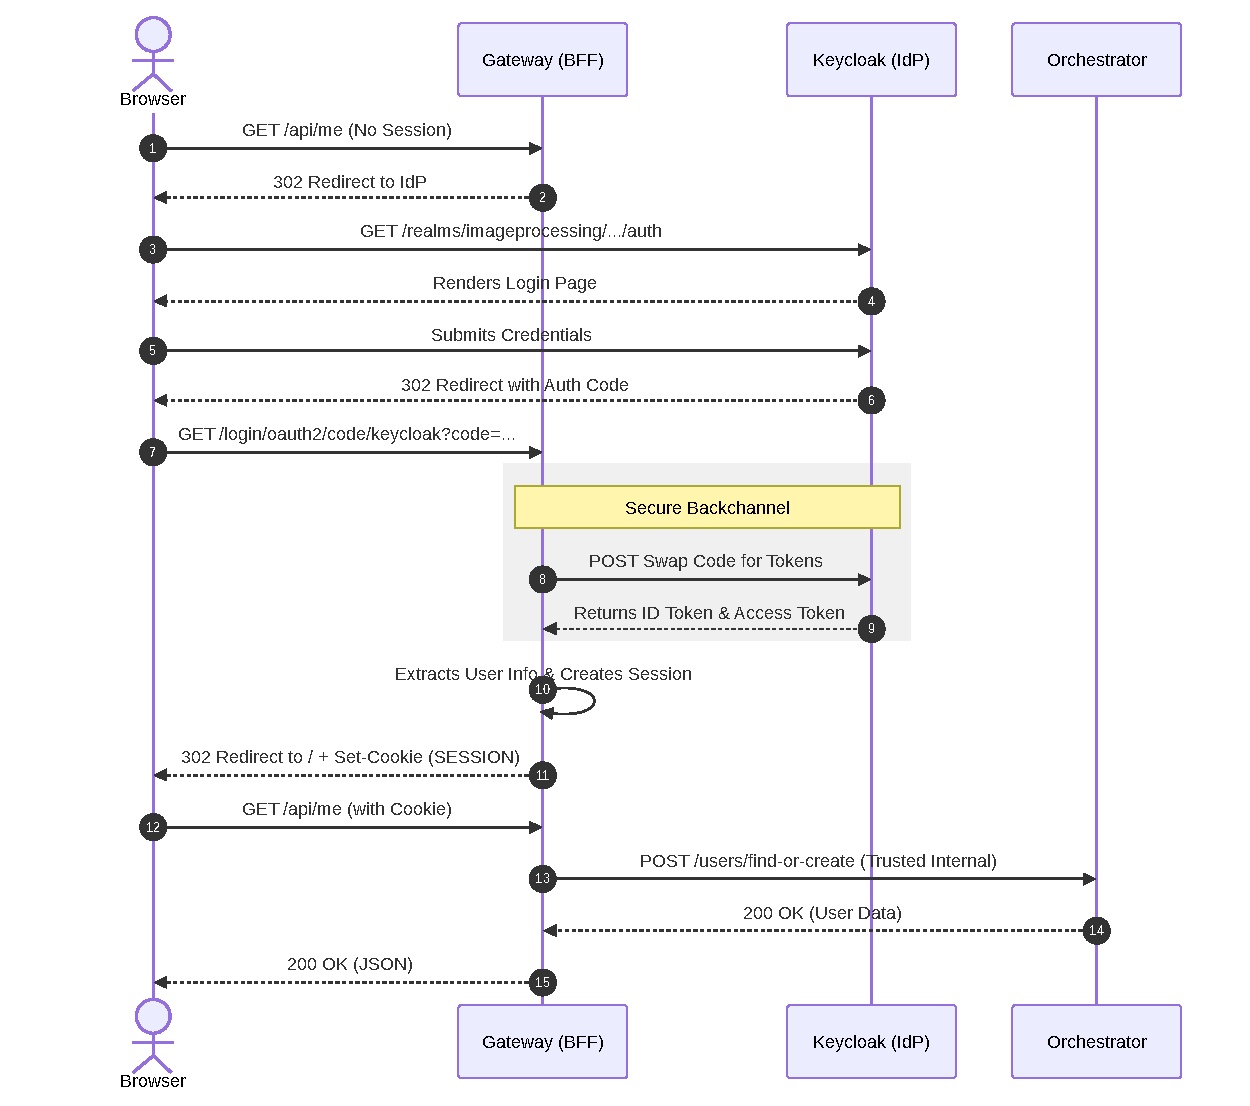
\includegraphics[width=\textwidth , height=0.85\textheight, keepaspectratio]{images/v5-oidc-sequence.pdf}
    \caption{OIDC login sequence diagram}
    \label{fig:v5-oidc-sequence}
\end{figure}

\subsection{Critical Assessment vs. Goal}
The authentication criterion, unauthenticated requests to protected endpoints rejected, is met, as is the event-driven identity-consistency criterion, now backed by a purpose-built event bridge rather than a generic polling or dual-write mechanism. The CI/CD criterion is met with one caveat stated plainly: the deploy step requires a manual trigger, not because of a design choice but because the target infrastructure (a personal laptop, not guaranteed to be online) makes a fully automatic deploy unreliable rather than unautomatable. This is a scope limitation of the environment, not of the pipeline design, and is revisited in Chapter \emph{Conclusions}.

\newpage

\section{Istio}

\subsection{Architecture}
The sixth milestone introduces a service mesh onto the Kubernetes deployment established in \emph{v4}, replacing point-to-point Kubernetes Services as the sole mechanism governing inter-service traffic with an Envoy-proxy-based mesh capable of L7-aware routing, weighted traffic splitting, and mesh-level resilience policy. Istio was installed via the \texttt{demo} profile rather than \texttt{default}, a deliberate choice given the single-node Minikube cluster's already-contended CPU budget across five application workloads, Postgres, and Kafka: the \texttt{demo} profile's more permissive default resource requests avoid the risk of mesh control-plane pods remaining perpetually \texttt{Pending} on a resource-constrained node. The NGINX Ingress Controller introduced in \emph{v4} was retired outright rather than run alongside the mesh: an Istio \texttt{Gateway} and matching \texttt{VirtualService} resources now own the external-to-cluster traffic path for both \texttt{api.imageprocessing.local} and \texttt{keycloak.imageprocessing.local}, ensuring a single, unambiguous owner of external routing for the remainder of this chapter, consistent with the precedent set in \emph{v4} of following whichever mechanism is authoritative on disk rather than retaining a superseded one alongside it.

% figure: v6 architecture flowchart (mesh topology: ingress gateway, sidecar-injected app tier, unmeshed data tier)
\begin{figure}[htbp]
    \centering
    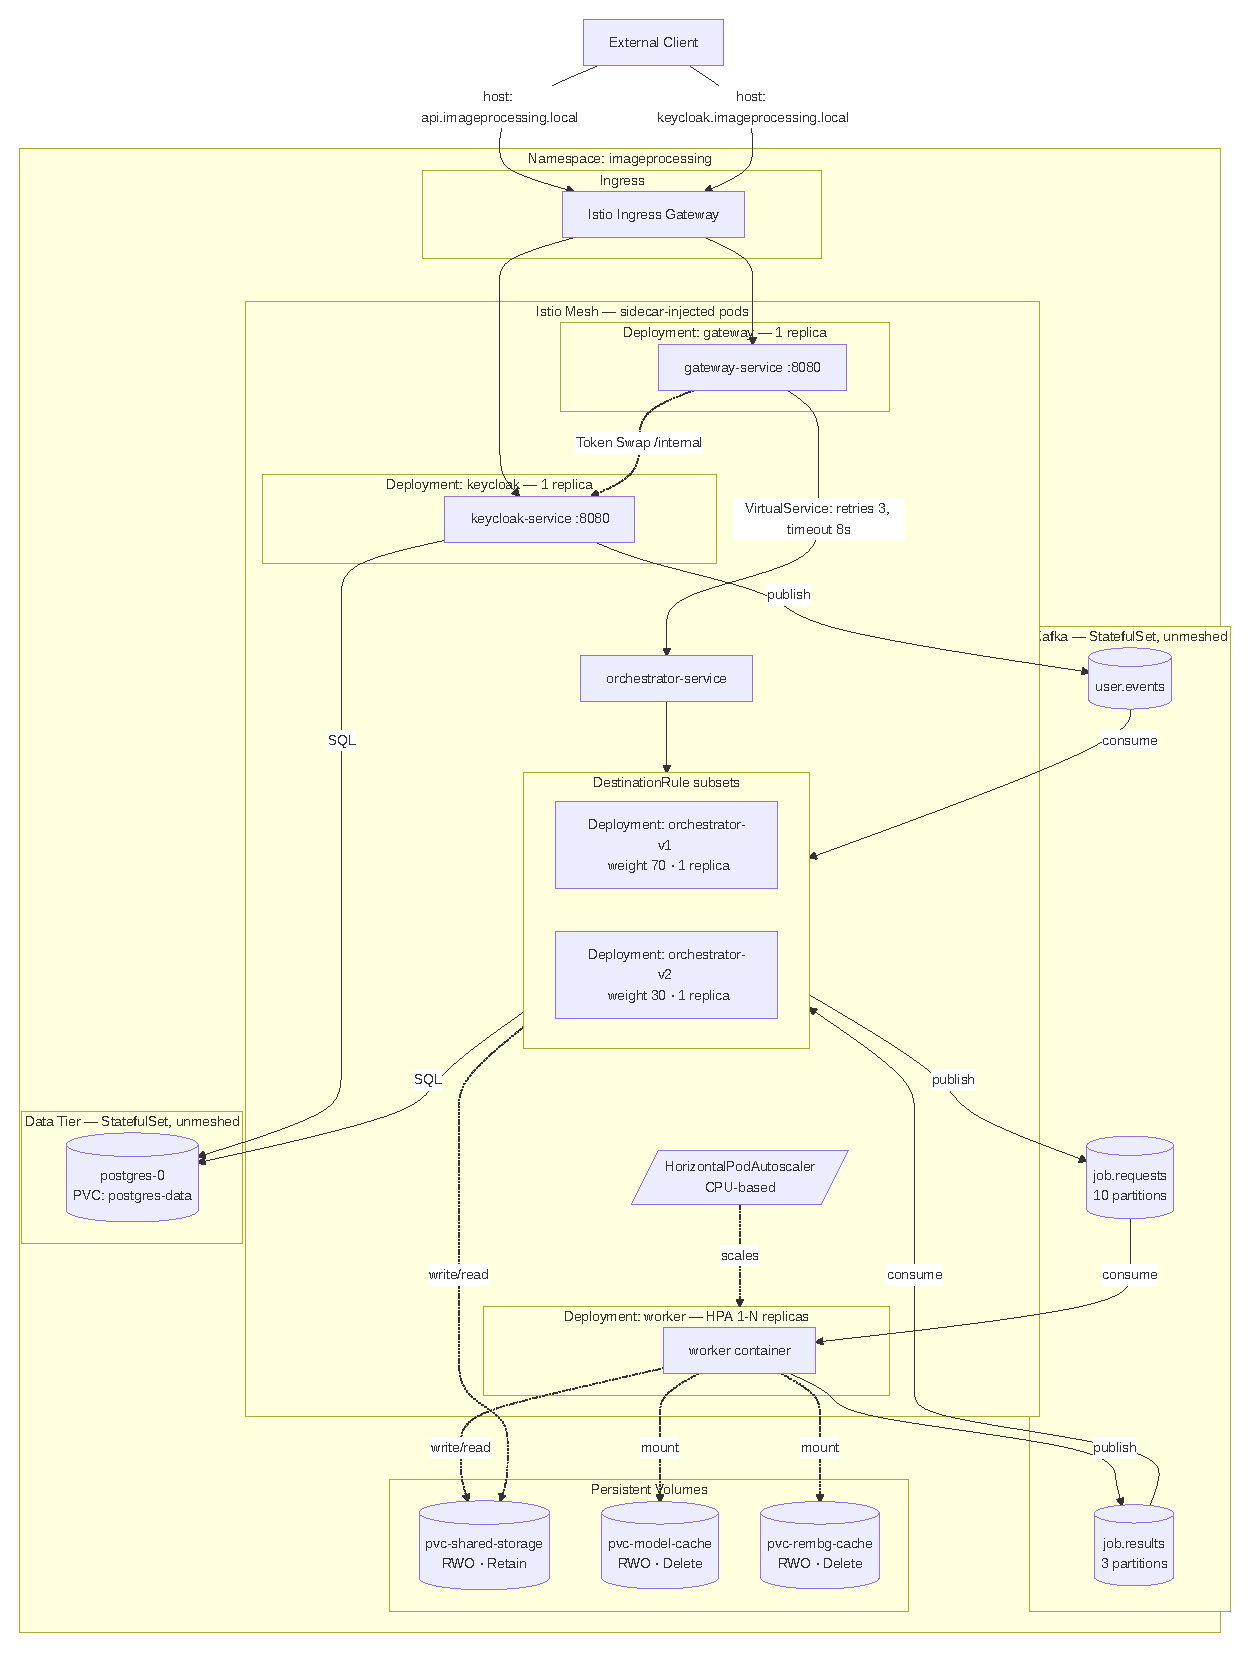
\includegraphics[width=\textwidth , height=0.85\textheight, keepaspectratio]{images/v6-architecture.pdf}
    \caption{Architecture flowchart (v6): Istio service mesh, sidecar injection scope, and weighted traffic management}
    \label{fig:v6-architecture}
\end{figure}

A deliberate scoping decision governs which workloads actually join the mesh. Sidecar injection is enabled at the namespace level for \texttt{imageprocessing}, meaning every pod scheduled into it receives an Envoy sidecar by default; Postgres and Kafka are explicitly excluded via a pod-level \texttt{sidecar.istio.io/inject: "false"} annotation, rather than left to accidental omission. Two considerations motivated this exclusion. First, both are StatefulSets with startup-ordering and DNS-resolution behavior already tuned across \emph{v3} and \emph{v4} (the \texttt{wait-for-postgres} init container, Kafka's KRaft controller-quorum voter addressing) around the assumption that the main container's own health, not a sidecar's, gates readiness; introducing a transparent proxy into that path would reopen startup-ordering questions already closed in earlier milestones, for no corresponding traffic-management benefit. Second, neither Postgres's wire protocol nor Kafka's is HTTP, so Istio's L7 routing, retry, and circuit-breaking primitives, the actual subject of this milestone, have nothing to act on for either service regardless. This is documented as a scoping decision open to revision, not a permanent architectural stance: meshing the data tier remains a candidate stretch item if the optional security milestone (mutual TLS between every service, including Postgres and Kafka) is pursued with time remaining.

\subsection{Application Structure and Development}
No new application code was introduced to support routing and resilience; the entirety of this milestone's core deliverable is expressed declaratively through Istio's Kubernetes-native custom resources, layered on top of the Deployments and Services already established in \emph{v4} and \emph{v5}. A \texttt{DestinationRule} for \texttt{orchestrator-service} defines a connection pool (\texttt{maxConnections}, \texttt{http1MaxPendingRequests}, \texttt{maxRequestsPerConnection}) and an outlier-detection policy (\texttt{consecutive5xxErrors}, \texttt{baseEjectionTime}, \texttt{maxEjectionPercent}); a companion \texttt{VirtualService} applies a request timeout and a bounded, status-code-scoped retry policy to the same hop. Both resources are intentionally scoped to the Frontend/Gateway \(\rightarrow\) Orchestrator hop specifically, rather than applied uniformly across every service pair in the system: the Orchestrator's other principal dependency, the AI Worker, has communicated exclusively over Kafka since the \emph{v4} messaging migration, so no HTTP hop exists there for Istio's L7 primitives to govern, and the Worker's consumer-group-based horizontal scaling is left entirely to Kafka's own partition-assignment protocol as before.

The milestone's second deliverable, a weighted canary split, required restructuring the Orchestrator from a single Deployment into two, \texttt{orchestrator-v1} and \texttt{orchestrator-v2}, sharing the existing \texttt{orchestrator-service}'s label selector (\texttt{app: orchestrator}) while carrying a distinguishing \texttt{version} label consumed only by Istio's \texttt{DestinationRule} \texttt{subsets}, not by the Kubernetes Service itself. This split deliberately keeps the two versions running from an identical container image: rather than introducing a genuine functional difference whose own correctness would need separate testing, effort orthogonal to this milestone's actual subject, the two versions are distinguished purely by an injected \texttt{INFO\_APP\_VERSION} environment variable surfaced through Spring Boot Actuator's \texttt{info} endpoint. This mirrors the project's stated stance, reiterated since the Thesis Proposal's Motivation section, that the object of evaluation is the surrounding orchestration, not the application logic being orchestrated. The corresponding \texttt{VirtualService} route splits traffic 70/30 across the two subsets, directly satisfying the relator-specified canary target, while retaining the same timeout and retry policy established for the non-canary configuration so that resilience behavior is not accidentally lost when weighted routing is introduced on top of it.

\subsection{Key Implementation Decisions}
Enabling the version-marker mechanism surfaced two implementation issues neither anticipated at design time, both worth recording as concrete findings rather than smoothed over as incidental setup noise. First, Spring Boot Actuator exposes only the \texttt{health} endpoint over HTTP by default; enabling \texttt{management.info.env.enabled} alone populates the \texttt{info} endpoint's contents but has no effect if the endpoint itself is never exposed via \\ \texttt{management.endpoints.web.exposure.include}. Requests to the unexposed endpoint did not fail with a clean \texttt{404}, but instead fell through to an unmatched wildcard route and surfaced as a generic \texttt{500}, a distinction made visible only by inspecting the request's Micrometer \texttt{Observation} log entry (\texttt{contextualName='http get /**'} rather than a concretely matched route). Second, and independently, \texttt{GlobalExceptionHandler}'s catch-all handler for unexpected exceptions had shipped since \emph{v1} with a \texttt{TODO} comment rather than an actual log statement, meaning every unanticipated server error had been silently opaque at the infrastructure layer for the life of the project until this milestone. Both gaps were fixed in the same rebuild: the missing exposure property was added, and the catch-all handler now logs the underlying exception before returning its uniform \texttt{ErrorResponse} body, closing a genuine observability gap that outlived five earlier milestones' worth of testing without being noticed.

A second, unrelated finding concerns the interaction between Istio's fault-injection and timeout mechanisms. An initial attempt to validate the configured \texttt{VirtualService} timeout by combining a synthetic \texttt{fault.delay} with a \texttt{timeout} field on the same HTTP route silently failed to demonstrate the intended behavior: a 10-second injected delay against a 5-second configured timeout completed successfully at the full 10 seconds rather than being cut off, a documented Envoy/Istio interaction in which fault injection and route-level timeout or retry policy do not co-apply on the same client-side route. Istio's own reference material sidesteps this by placing the delay and the timeout on two different services' \texttt{VirtualService} resources in a multi-hop call chain; this architecture has exactly one meshed HTTP hop of interest, so that decoupling was not structurally available without introducing \texttt{EnvoyFilter}-based fault injection at the destination's inbound listener, judged out of proportion to this milestone's traffic-management priority and left as an explicit, stated gap rather than pursued further.

Finally, the Orchestrator's outlier-detection configuration deliberately sets \\ \texttt{maxEjectionPercent} to 100, a value that would be considered aggressive against a genuinely load-balanced pool of replicas but is the only sensible choice here: the Orchestrator runs as a single replica throughout this project (Table~\ref{tab:architectural-evolution}), so Istio's conservative default of ejecting no more than 10\% of a pool would, in effect, refuse to ever eject the only member. This choice was validated directly rather than assumed: deliberately inducing failures against both canary subsets simultaneously (see \emph{Validation} below) confirmed that the mesh does eject a fully unhealthy backend at this setting rather than continuing to route traffic into it.

\subsection{Validation}
Each resilience mechanism introduced in this milestone was validated with a targeted, reproducible experiment rather than assumed correct from the declared configuration alone, following the same evidentiary standard established in earlier chapters (the k6 load test in \emph{v4}, the infrastructure audit script in \emph{v3}).

\textbf{Fault-injection capability.} A synthetic 3-second delay injected via \texttt{VirtualService} \\ \texttt{fault.delay}, with no competing \texttt{timeout} field on the same route, produced a wall-clock request time of 3.01 seconds against an otherwise-instant health endpoint, confirming that Envoy genuinely intercepts and delays traffic on command.

\textbf{Circuit breaking under load.} With the Orchestrator's connection pool deliberately tightened (\texttt{http1MaxPendingRequests: 2}, \texttt{maxRequestsPerConnection: 1}), 60 concurrent in-mesh requests produced 50 rejections and 10 successes; every rejected response carried Envoy's \texttt{x-envoy-overloaded: true} header, and every successful response carried a genuine upstream service time, ruling out the possibility that the observed failures were coincidental application-level errors rather than the connection-pool circuit breaker itself.

\textbf{Fail-fast behavior against a fully unavailable backend.} Scaling the Orchestrator to zero replicas produced an immediate (0.01 second) \texttt{503} carrying the body \\ \texttt{no healthy upstream}, rather than a hang. This result is reported precisely rather than over-claimed: the near-instant failure reflects Envoy's endpoint-discovery layer recognizing zero available endpoints at the routing layer, not the configured \texttt{timeout} value being reached, and outlier detection's defining behavior, ejecting one failing replica from a pool while others continue serving, remains unproven against this architecture's single-replica Orchestrator for the same reason already acknowledged for the Worker's untested 10-replica scheduling ceiling in \emph{v4}.

\textbf{Weighted canary routing.} Ten thousand sequential requests against the split Orchestrator subsets returned 7{,}061 responses tagged \texttt{v1} and 2{,}939 tagged \texttt{v2}, a 70.61\%/29.39\% observed split against a configured 70/30 target, a 0.61-percentage-point deviation attributable to the expected variance of Envoy's weighted round-robin implementation at this sample size. Reaching this result required first diagnosing an unrelated failure: an initial run against the same configuration returned \texttt{no healthy upstream} for 498 of 500 requests, traced not to a routing misconfiguration but to both canary subsets sharing the same latent Actuator exposure bug described above, which caused Phase 1's own outlier detection to correctly eject both endpoints in quick succession once each accumulated five consecutive real failures. Resolving the underlying application bug, rather than adjusting the mesh configuration, restored the expected split immediately, itself a demonstration that the resilience machinery introduced earlier in this milestone was operating exactly as designed even before the canary feature was validated on top of it.

\subsection{Critical Assessment vs. Goal}
Against the two success criteria the relator identified as highest priority for this milestone, traffic management and canary deployment, both are met with direct, quantified evidence rather than declarative configuration alone: weighted routing, connection-pool circuit breaking, and request timeout/retry policy are each independently validated in isolation, and the 70/30 canary split is demonstrated at a sample size large enough to distinguish a correctly-configured split from a coincidental one. The success criterion stated in Chapter \emph{Goal} for this milestone, that \emph{"a simulated failure in one service is contained by mesh-level retry/circuit-breaking policy without requiring a code change in the calling service,"} is satisfied concretely: the circuit-breaker and fail-fast experiments above were both conducted, and passed, without touching the Frontend/Gateway's own code at all.

The remaining criterion, that \emph{"service-to-service traffic is encrypted and policy-controlled at the mesh level"} (mutual TLS and \texttt{AuthorizationPolicy}), was explicitly scoped as optional by the relator and was not pursued in the time available, consistent with the milestone's own stated priority ordering (traffic management, most important; canary, second; security and policy configuration, optional). This is recorded here as a deliberate, acknowledged scope boundary rather than an oversight: the mesh's sidecar topology and existing \texttt{DestinationRule}/\texttt{VirtualService} resources for the Orchestrator hop would extend cleanly to carry a \texttt{PeerAuthentication} and \texttt{AuthorizationPolicy} pair if pursued, since both build on infrastructure already in place from this chapter, but doing so was judged secondary to delivering the two higher-priority deliverables with genuine, load-tested evidence rather than spreading the remaining time across a larger surface with shallower validation on each part.


\section{Cross-Cutting Results}

\subsection{Observability Implementation}
Observability instrumentation was established early and deliberately kept ahead of the infrastructure needed to consume it. From the first milestone, critical service and storage methods are annotated with Micrometer's \texttt{@Observed}, which produces traces and metrics regardless of whether a backend is present to receive them; this is a conscious choice to bake instrumentation into the application code as a baseline concern from the outset, rather than retrofitting it once a monitoring stack exists to make it visible.

This instrumentation was made async-aware from the same milestone, rather than left to silently break once background execution was introduced. Micrometer's tracing instrumentation stores the current trace context in a thread-local variable, which does not automatically carry over when execution hops to a different thread, a problem the monolith's job-execution model hits directly, since \texttt{ProcessingJobService.startAsyncProcessExecution} runs on a separate \texttt{@Async} executor thread rather than the HTTP-handling thread that received the original request. Left unaddressed, this would have produced two disconnected traces per job, one for the synchronous request that created it, and an orphaned one for its actual execution, rather than a single trace spanning the job's full lifecycle. This was resolved by registering Spring's \texttt{ContextPropagatingTaskDecorator} on the \texttt{@Async} executor configured in \texttt{AsyncConfig}, which copies the trace context onto the new thread before the async task runs, so that a job's asynchronous execution appears as a continuation of the same trace as the request that triggered it. This decision, made in \emph{v1} before there was any distributed system to speak of, paid off directly once the architecture actually became distributed: the same propagation concern reappears, structurally unchanged, at the Kafka publish/consume boundary introduced in \emph{v4}, where a trace must again survive a hop across an asynchronous execution boundary, this time a message queue rather than a thread pool.

At the time of writing, this instrumentation baseline is only partially consumed: the Orchestrator's logs report an expected, explicitly-anticipated \texttt{"Failed to publish metrics to OTLP receiver"} warning, since no OpenTelemetry collector is deployed yet. This is not treated as an unnoticed defect but as a known, deferred gap: full consumption of the existing \texttt{@Observed} instrumentation, distributed tracing via Jaeger, metrics collection via Prometheus, dashboarding via Grafana, and service-topology visualization via Kiali, is of the service mesh milestone (\emph{v6}), where Istio's sidecar model provides a natural point at which to deploy the surrounding collection stack. The instrumentation groundwork, including the async-context-propagation concern that will matter most once traces must be reconstructed across service boundaries, having already been laid in \emph{v1} rather than deferred alongside the collection stack itself, means this milestone's remaining work is deployment and wiring, not re-instrumentation of application code.

\subsection{Secrets Management in Practice}
The secrets-management pattern described in Chapter \emph{Approach} recurs concretely at every layer of the deployed system. Locally, database credentials live in a git-ignored \\ \texttt{application-local.properties}, activated via Spring profiles, with a committed template guiding setup. In the containerized environment, an excluded \texttt{.env} file supplies \\ \texttt{POSTGRES\_USER}, \texttt{POSTGRES\_PASSWORD}, and storage paths to Docker Compose. In the cluster, PostgreSQL's credentials are held in a single \texttt{postgres-secret}, with a committed \texttt{secret.example.yml} as the onboarding template; because the official Postgres image hardcodes \texttt{POSTGRES\_USER}/\texttt{POSTGRES\_PASSWORD} while Spring Boot expects \\ \texttt{POSTGRES\_USER\_NAME}/\texttt{POSTGRES\_USER\_PASSWORD}, the same secret is consumed under two different key-mapping strategies, a blanket \texttt{envFrom} for Postgres itself, and explicit \\ \texttt{secretKeyRef} mappings for the Orchestrator, rather than maintaining two secrets with duplicated values. The same resolution was reused verbatim for Keycloak's database credentials in \emph{v5}, rather than re-solved independently. Finally, registry authentication for the CI/CD pipeline uses a purpose-scoped GitLab Deploy Token (\texttt{read\_registry} only) rather than a personal account credential, mounted into the cluster as a \texttt{gitlab-registry-secret}, limiting what a compromised pipeline or leaked credential could actually access.

\subsection{Known Limitations}
The CI/CD pipeline itself matured incrementally across the project rather than appearing fully-formed at \emph{v5}: the test and build stages were established first, against locally-built images, and only later extended to deploy against the live cluster once the runner and registry-authentication constraints (Chapter \emph{Results}, Section \emph{Keycloak/Auth}) were resolved.

A small number of known limitations were surfaced across \emph{v4} and \emph{v5} and remain open at the time of writing, carried forward here explicitly as part of the current to-be state rather than deferred silently to the conclusions:

\begin{itemize}
    \item \textbf{Shared storage remains single-node-only.} The shared storage \texttt{PersistentVolume} is declared \texttt{ReadWriteOnce} against a \texttt{hostPath} backend, an honest reflection of what \texttt{hostPath} can actually enforce (Chapter \emph{Results}, Section \emph{Kubernetes}), but this constrains the cluster to a single node until migration to a genuine \texttt{ReadWriteMany} backend (NFS or a cloud file share).
    \item \textbf{ML model-cache PVCs carry the same unaddressed multi-node risk} as the shared storage volume did before its relabeling, since they remain \texttt{ReadWriteOnce} against the same \texttt{standard} StorageClass; baking the models into the Worker image at build time, rather than caching them at runtime, is the identified candidate fix.
    \item \textbf{The Worker's schedulability at the full 10-replica autoscaling ceiling remains unvalidated.} Only a CPU request (\texttt{200m}) is configured on the Worker container, with no memory request or limit of any kind; the KEDA/Kafka trigger logic itself was proven correct (Chapter \emph{Results}, Section \emph{Kubernetes}), but whether the underlying Minikube node has the capacity to actually schedule 10 concurrent Worker replicas was never load-tested to that ceiling.
    \item \textbf{The CI/CD deploy stage requires a manual trigger.} This follows from the target infrastructure, a personal laptop not guaranteed to be online, rather than from the pipeline's design; the architecturally preferable pull-based mechanism (GitLab Agent for Kubernetes) remains blocked by a server-side instance misconfiguration outside the project's control.
    \item \textbf{CSRF protection is disabled at the Gateway}, a direct consequence of the static frontend having no templating engine through which to inject per-request tokens (Chapter \emph{Results}, Section \emph{Keycloak/Auth}); acceptable for a single-origin, thesis-scale deployment, but not a pattern to carry forward without revisiting if the frontend or deployment topology changes.
\end{itemize}

None of these limitations affect the validated behavior of any individual milestone in isolation, but they bound the claims that can be made about the system's behavior at full scale or in a hardened production setting, and are revisited in Chapter \emph{Conclusions}.

\chapter{Conclusions}

\section{Goals Achieved}
Measured against the success criteria defined in Chapter \emph{Goal}, five of the six planned milestones are complete and independently validated, and the sixth is complete against its two relator-specified mandatory priorities.

\textbf{Monolith (\emph{v1}).} A complete REST API over a three-entity domain model (\texttt{User}, \texttt{Image}, \texttt{ProcessingJob}), with an end-to-end processing job, upload, process, download, completing and being automatically testable without manual intervention, as required. The \texttt{ImageService}/\texttt{ImageProcessor} boundary, designed from the outset to anticipate a future service split, paid off directly and without restructuring in both \emph{v2} and \emph{v4}.

\textbf{Microservices (\emph{v2}).} The AI Worker deployable, restartable, and independently scalable from the Gateway and Orchestrator, with no shared process or failure domain, validated by a stateful, concurrent end-to-end pytest suite exercising all three job types in parallel against all three services.

\textbf{Containerization (\emph{v3}).} Every custom service builds and runs as a non-root container; the full four-container stack starts from a single \texttt{docker compose up}; both criteria independently confirmed by the automated \texttt{validate\_infra.sh} audit rather than by inspection alone.

\textbf{Kubernetes (\emph{v4}).} The system survives arbitrary pod deletion without manual intervention (Deployments and StatefulSets replacing bare Pods); the Worker scales automatically under load; a full deployment reaches the cluster without manually copying files or images onto the target machine. Five workloads across two controller types, Kafka providing thread decoupling and load buffering for the Orchestrator-to-Worker hop, and elastic scaling explored via both KEDA (1-10 replicas, Kafka-lag-driven) and, per relator direction favoring curriculum alignment, standard CPU-based HPA as the mechanism carried into the final deployment.

\textbf{Keycloak/Auth (\emph{v5}).} Unauthenticated requests to protected endpoints are rejected; user deletion in Keycloak propagates to the Orchestrator's domain data through an event-driven Kafka bridge rather than a synchronous, tightly-coupled call; a pushed code change reaches the running cluster through the CI/CD pipeline with only the final deploy trigger performed manually, a constraint of the target infrastructure (Chapter \emph{Results}, Keycloak/Auth) rather than of the pipeline's design.

\textbf{Istio (\emph{v6}).} Against the relator's stated priority ordering, traffic management (most important) and canary deployment (second priority) are both complete with quantified, load-tested evidence: a connection-pool circuit breaker rejecting 50 of 60 concurrent requests under a deliberately tightened pool, each rejection independently confirmed via Envoy's \texttt{x-envoy-overloaded} flag; a weighted canary split measured at 70.61\%/29.39\% against a configured 70/30 target across ten thousand requests; and a simulated single-service failure contained entirely by mesh-level policy with no code change in the calling service, directly satisfying the corresponding Goal-chapter criterion. Security and policy configuration at the mesh level, explicitly marked optional by the relator, were not pursued within the available time and are addressed in the following section.

\section{Goals Not Reached / Deferred}
\textbf{Istio security and policy configuration.} Mutual TLS (\texttt{PeerAuthentication}) and service-to-service authorization (\texttt{AuthorizationPolicy}) were scoped as optional from the outset of the milestone and were not implemented. This was a deliberate allocation of the remaining time toward deeper, load-tested validation of the two mandatory deliverables rather than shallower coverage spread across a wider surface; the mesh's existing sidecar topology and \texttt{DestinationRule}/\texttt{VirtualService} resources for the Orchestrator hop would extend to carry these policies without structural rework, should the milestone be revisited.

\textbf{Infrastructure as Code (Terraform/Ansible).} Identified as a stretch goal at the project's outset, conditional on time remaining after the core \emph{v1}-\emph{v6} roadmap. It was not pursued. Had it been, the expected benefit would have been reproducible provisioning of the cloud cluster, VPC networking, and storage buckets described in the Thesis Proposal, removing the manual \texttt{minikube start}/\texttt{eval \$(minikube docker-env)} sequence as a source of environment drift between the developer's machine and any future teaching replication of this project; the benefit is judged real but strictly additive to, not a precondition for, the milestones actually delivered.

\textbf{Open follow-ups surfaced during \emph{v4} and \emph{v5}, still outstanding.} The shared-storage \texttt{PersistentVolume} remains \texttt{ReadWriteOnce} against a \texttt{hostPath} backend, an honest reflection of what \texttt{hostPath} can enforce rather than the \texttt{ReadWriteMany} guarantee a genuinely multi-node deployment would need; the ML model-cache PVCs carry the same unaddressed constraint. The Worker's schedulability at KEDA's full ten-replica ceiling was never validated against real CPU/memory resource requests on the underlying node. The CI/CD deploy stage remains a manually-triggered rollout restart rather than a fully automatic one, a consequence of the GitLab Agent for Kubernetes being blocked instance-wide by a server-side misconfiguration outside the project's control, not a limitation of the pipeline's own design.

\textbf{A new, milestone-specific gap surfaced during Istio validation.} The Sprint 3 k6 load test (\texttt{test/loadtest.js}) was discovered, while validating the \emph{v6} circuit breaker, to be non-functional against the system as it exists after \emph{v5}: its \texttt{setup()} phase calls \texttt{POST /api/users} through the public Gateway, a route that has been behind Keycloak's OIDC authentication filter since \emph{v5} and that the script has no mechanism to satisfy. This had gone unnoticed for an entire milestone because no regression run against it had been attempted between \emph{v5}'s completion and \emph{v6}'s validation work; it is recorded here explicitly as a gap in this project's own regression discipline, not only as a defect in the script.

\section{Critical Reflection}
The validation strategy adopted across this project, automated test suites, an infrastructure audit script, a k6 load profile, and, in this final milestone, targeted fault-injection and load-driven experiments against declared mesh policy, was chosen specifically to avoid asserting that infrastructure behaves as configured without evidence that it does. Several results bear this out directly. The Kafka migration's central claim, thread decoupling and load buffering for the Orchestrator, is architecturally motivated rather than independently load-tested against a saturating burst in this project, an honest limit worth stating rather than implying stronger evidence than exists. KEDA's Kafka-lag-driven scaling, by contrast, was directly demonstrated against a synthetic 30-message burst driving the expected \(\lceil 30/10 \rceil = 3\) replicas, a concrete, quantified confirmation of the backlog-based-versus-proxy-metric argument made in Chapter \emph{State of the Art} for why lag is a better scaling signal than CPU for a bursty, queue-fed worker, even though CPU-based HPA was the mechanism ultimately carried into the final deployment for curriculum-alignment reasons.

The Istio milestone's validation is, on reflection, the most rigorously evidenced of the six: every mechanism claimed, fault-injection capability, connection-pool circuit breaking, fail-fast behavior against a fully unavailable backend, and weighted canary routing, was measured with a specific, reproducible experiment and a recorded number, rather than inferred from a successfully-applied YAML manifest. This rigor also surfaced two results worth weighing honestly rather than only celebrating. First, an attempted combined test of fault-delay injection and route timeout returned a false negative, later understood as a documented Envoy/Istio interaction rather than a configuration error, a reminder that infrastructure behavior can defeat an intuitively reasonable test design even when both the system under test and the test itself are individually correct. Second, the canary validation's first real attempt failed almost completely, not because the mesh configuration was wrong, but because a five-milestone-old, previously undetected gap, \texttt{GlobalExceptionHandler}'s catch-all exception handler shipping since \emph{v1} with a logging statement left as a \texttt{TODO} rather than implemented, made an unrelated application bug indistinguishable from an infrastructure fault until the logs were manually inspected in detail. That the milestone's own resilience mechanism, outlier detection, correctly and automatically ejected both failing endpoints during this incident is a genuine, if unplanned, demonstration that the mechanism works exactly as designed; that the underlying bug had been invisible for five milestones is a genuine, and separately important, finding about the cost of deferred observability work.

\section{Generalizability and Future Work}
Several aspects of this work extend beyond the specific coursework context in which it was produced. The institutional CI/CD constraints encountered in \emph{v5}, no Docker-in-Docker on shared runners, a blocked pull-based deployment agent, are a recognized and generalizable class of problem in academic and other resource-constrained CI environments, not specific to this project's infrastructure; the interim solutions adopted here, daemonless image building via Kaniko and a project-specific shell-executor runner, are documented with their tradeoffs stated explicitly (Chapter \emph{Approach}, Security and Secrets Management Strategy) precisely so that the choice, and its limits, transfer to a similar future situation rather than being read as a universally-recommended pattern. The progressive, milestone-driven decomposition methodology itself, monolith before microservices, microservices before containerization, containerization before orchestration, messaging before elastic scaling, identity before service mesh, is offered as a teaching pattern in its own right: each transition in Table~\ref{tab:architectural-evolution} was deliberately sequenced so that the concept introduced at one stage remained a stable precondition for the next, rather than several concerns being introduced simultaneously and confounded in a student's understanding of which change caused which effect.

Concrete future work follows directly from the gaps recorded above: completing Istio's optional security and policy configuration (\texttt{PeerAuthentication}, \texttt{AuthorizationPolicy}) on the existing mesh topology; migrating shared and model-cache storage to a genuine \texttt{ReadWriteMany} backend before any multi-node cluster is introduced; establishing real CPU/memory resource requests on the Worker and validating the ten-replica KEDA ceiling against them; repairing the k6 load test's authentication gap so it can resume serving as a regression check; and, smaller but concretely actionable, extending the exception-logging fix made during \emph{v6} (\texttt{GlobalExceptionHandler} now logging unexpected exceptions rather than silently swallowing them) as a review checklist item for any future catch-all handler added to the codebase. The bonus Infrastructure-as-Code track (Terraform, Ansible) remains available as a natural next extension of the cloud-provisioning phase referenced in the original roadmap.

\section{Limits}
This thesis does not claim to have conducted a production-grade security audit of the resulting system: CSRF protection is disabled at the Gateway by explicit, documented design choice (Chapter \emph{Results}, Keycloak/Auth), and Istio's mutual-TLS and authorization capabilities, while architecturally available, were not enabled. It does not claim performance validated against industry-scale baselines; every load figure reported in this document, the k6 profile's five concurrent virtual users, the circuit-breaker test's sixty concurrent requests, the canary validation's ten thousand sequential requests, was sized to produce a clear, statistically legible signal at thesis scale, not to characterize behavior under production traffic volumes. The deployment target throughout is a single-node Minikube cluster; several design decisions, the shared-storage volume's \texttt{ReadWriteOnce} access mode chief among them, are stated honestly as correct \emph{for a single node} and explicitly not yet validated for a genuinely distributed, multi-node deployment. Finally, this project was executed by a solo developer under thesis-scale constraints: the CI/CD deploy stage's shell-executor runner, granting job scripts direct access to the developer's own machine, is explicitly flagged in Chapter \emph{Approach} as an accepted tradeoff for exactly this reason, and is not recommended as a pattern for any setup with multiple contributors pushing to the same pipeline.

\appendix

\chapter{Thesis Proposal}
\label{app:thesis-proposal}

\includepdf[pages=-, scale=0.8, pagecommand={}]{images/thesis-proposal.pdf}

\chapter{Proposed Architecture Diagram}
\label{app:proposed-architecture-diagram}
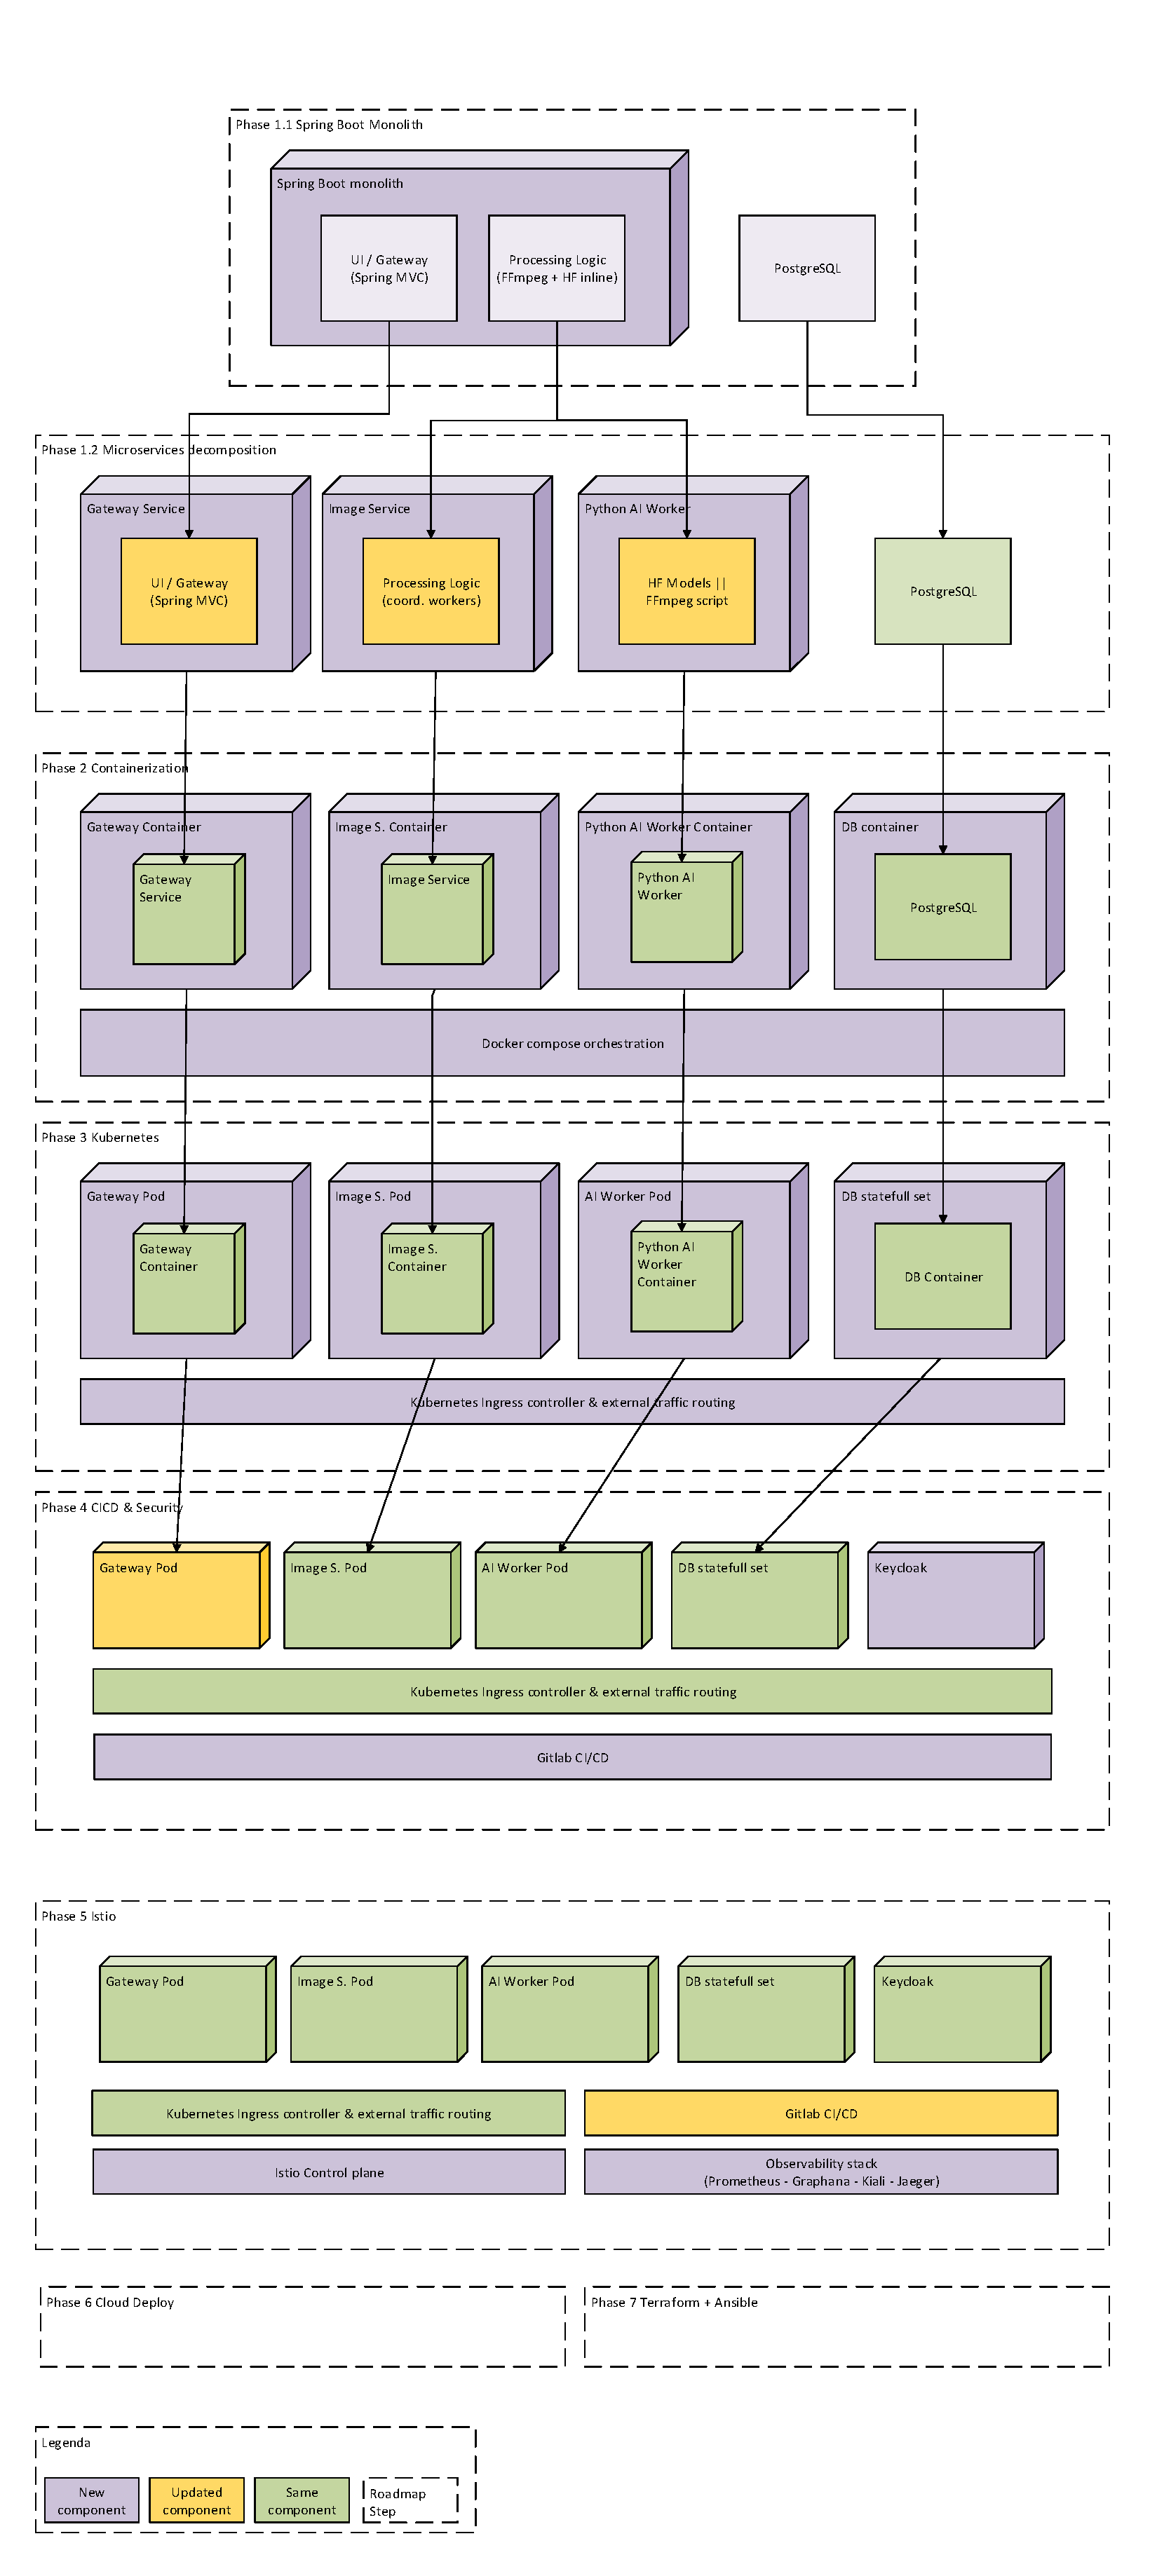
\includepdf[pages=-, scale=0.8, pagecommand={}]{images/thesis-architecture.pdf}

\bibliographystyle{unsrt}
\bibliography{bibliografia}
\end{document}
